\section{Annexes}

Graficos de referencia inicial:

\section{A case}

\begin{figure}[H]
  \centering
  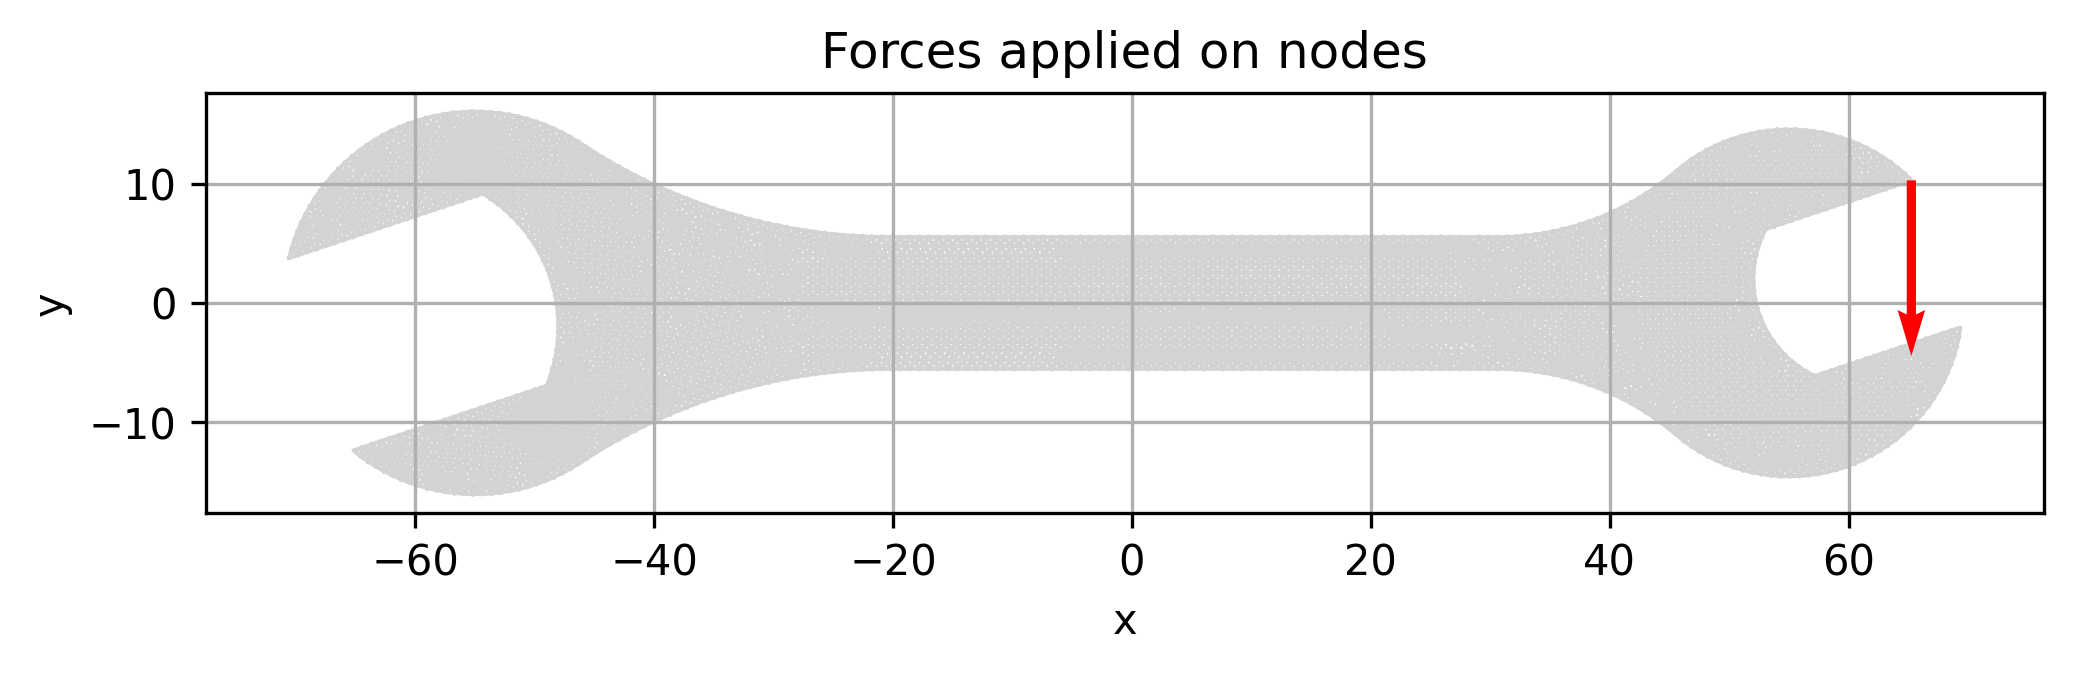
\includegraphics[width=0.8\textwidth]{GRAFICOS/Case a_fuerzas.png}
  \caption{Caption}
  \label{fig:strain}
\end{figure}

\begin{figure}[H]
  \centering
  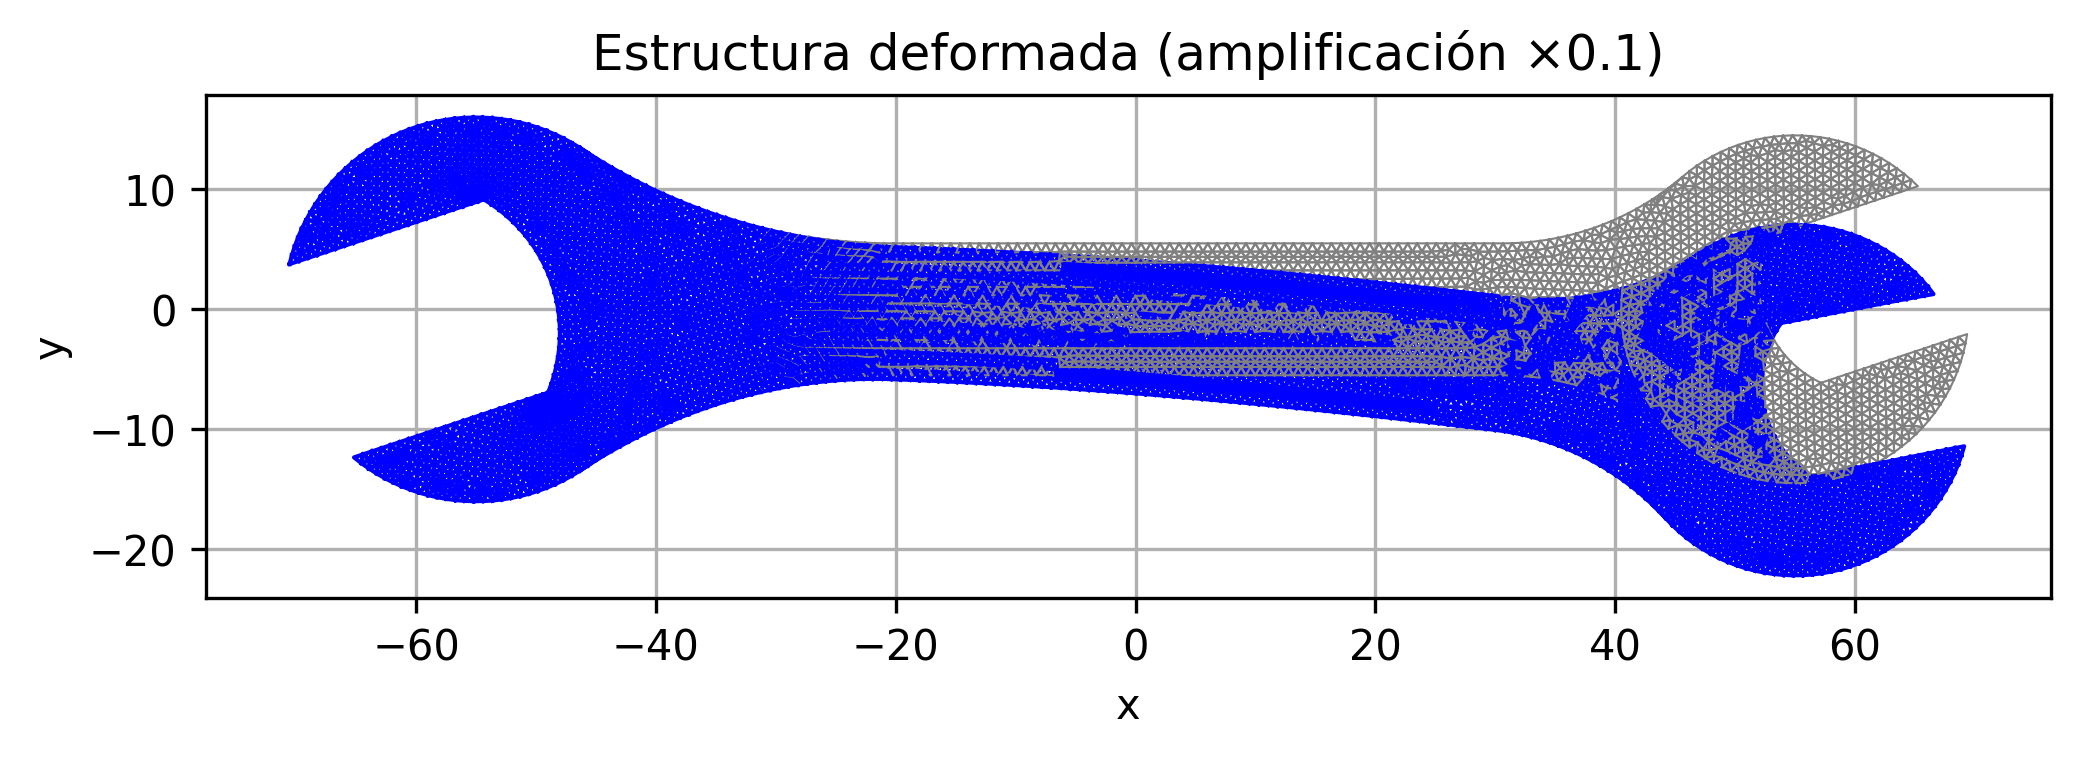
\includegraphics[width=0.8\textwidth]{GRAFICOS/Case a_deformada.png}
  \caption{Caption}
  \label{fig:stress}
\end{figure}

\begin{figure}[H]
  \centering
  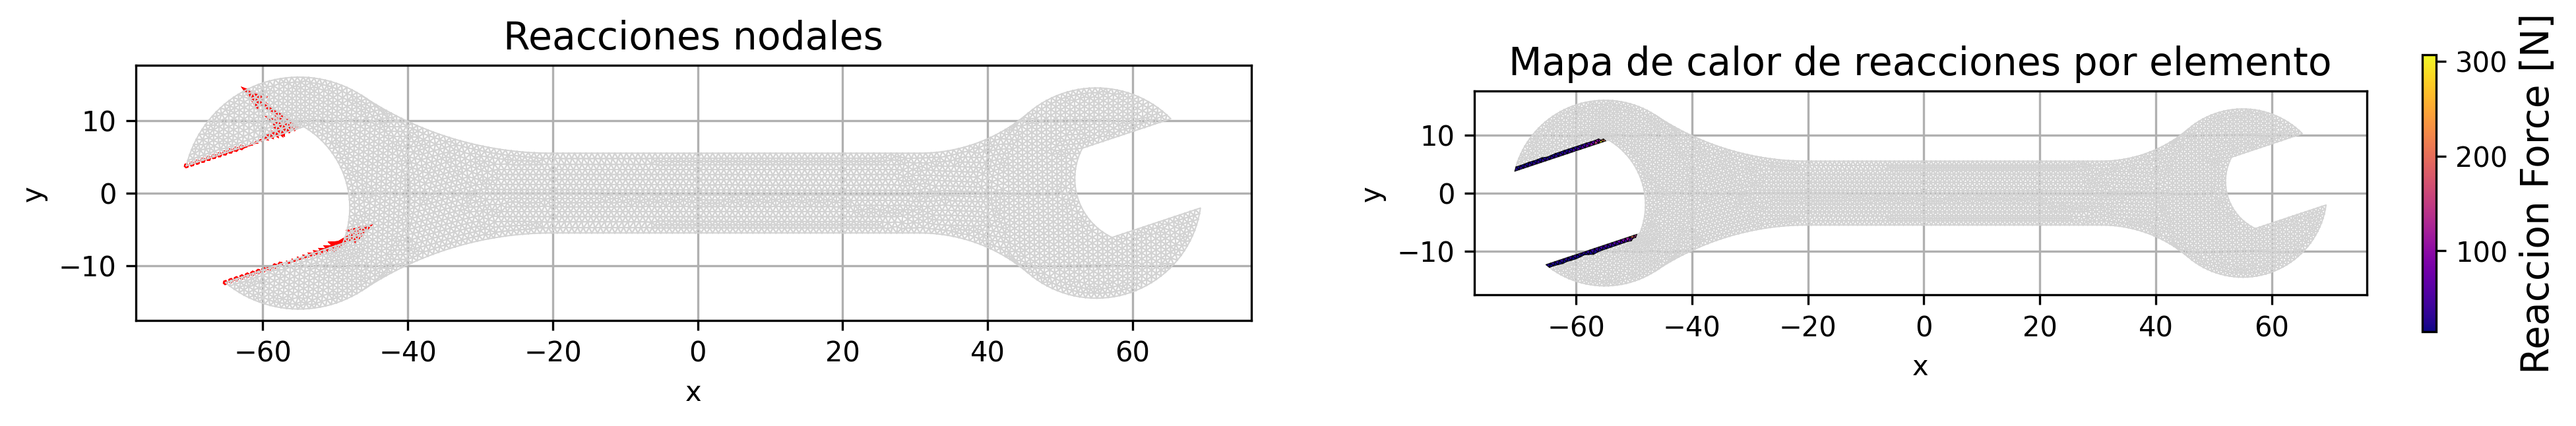
\includegraphics[width=1\textwidth]{GRAFICOS/Case a_deformada_reacciones.png}
  \caption{Caption}
  \label{fig:principal}
\end{figure}

\begin{figure}[H]
  \centering
  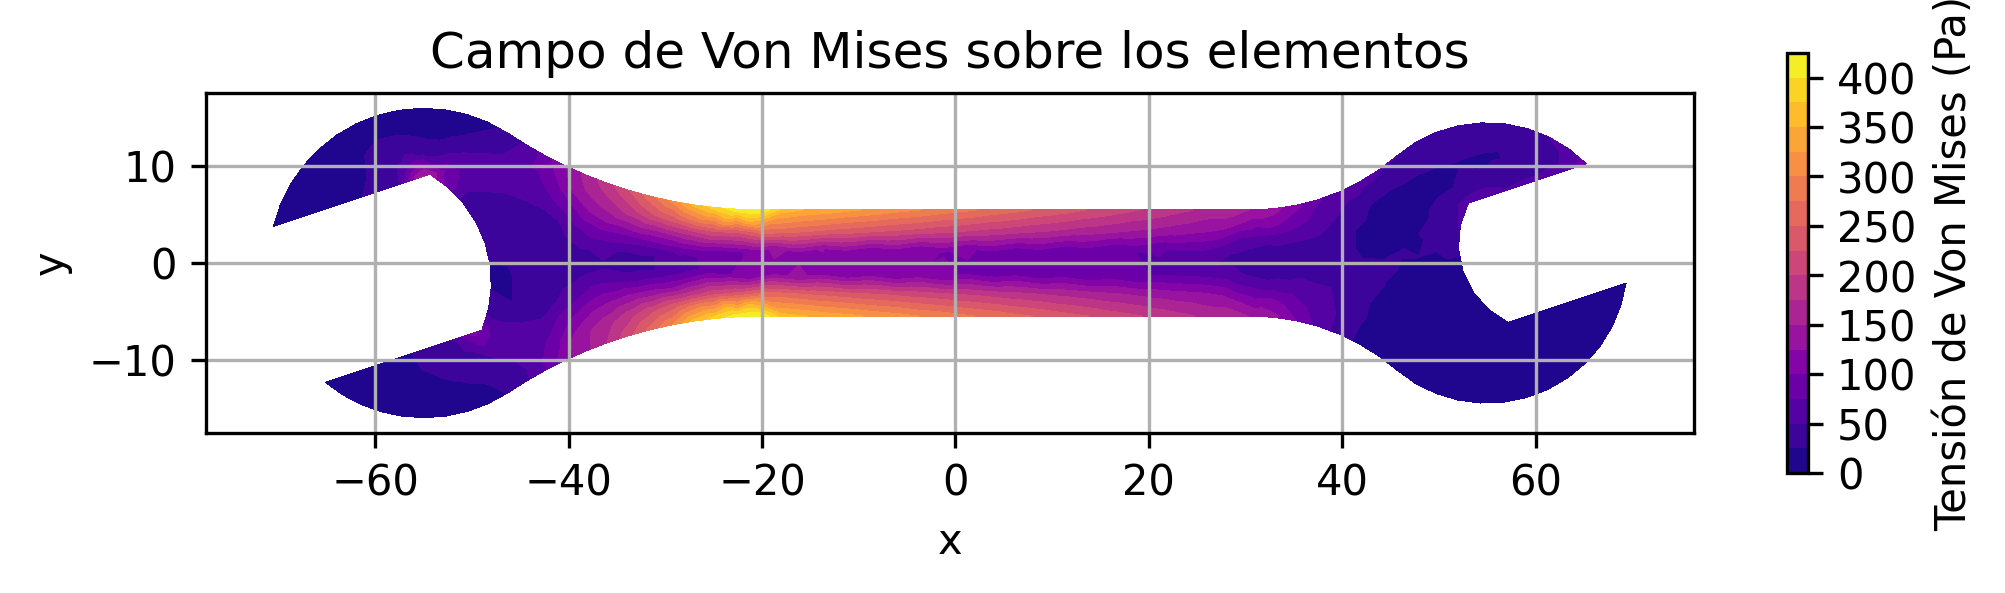
\includegraphics[width=0.8\textwidth]{GRAFICOS/Case a_von_mises.png}
  \caption{Caption}
  \label{fig:principal}
\end{figure}

\begin{figure}[H]
  \centering
  \begin{subfigure}[t]{0.49\textwidth}
    \centering
    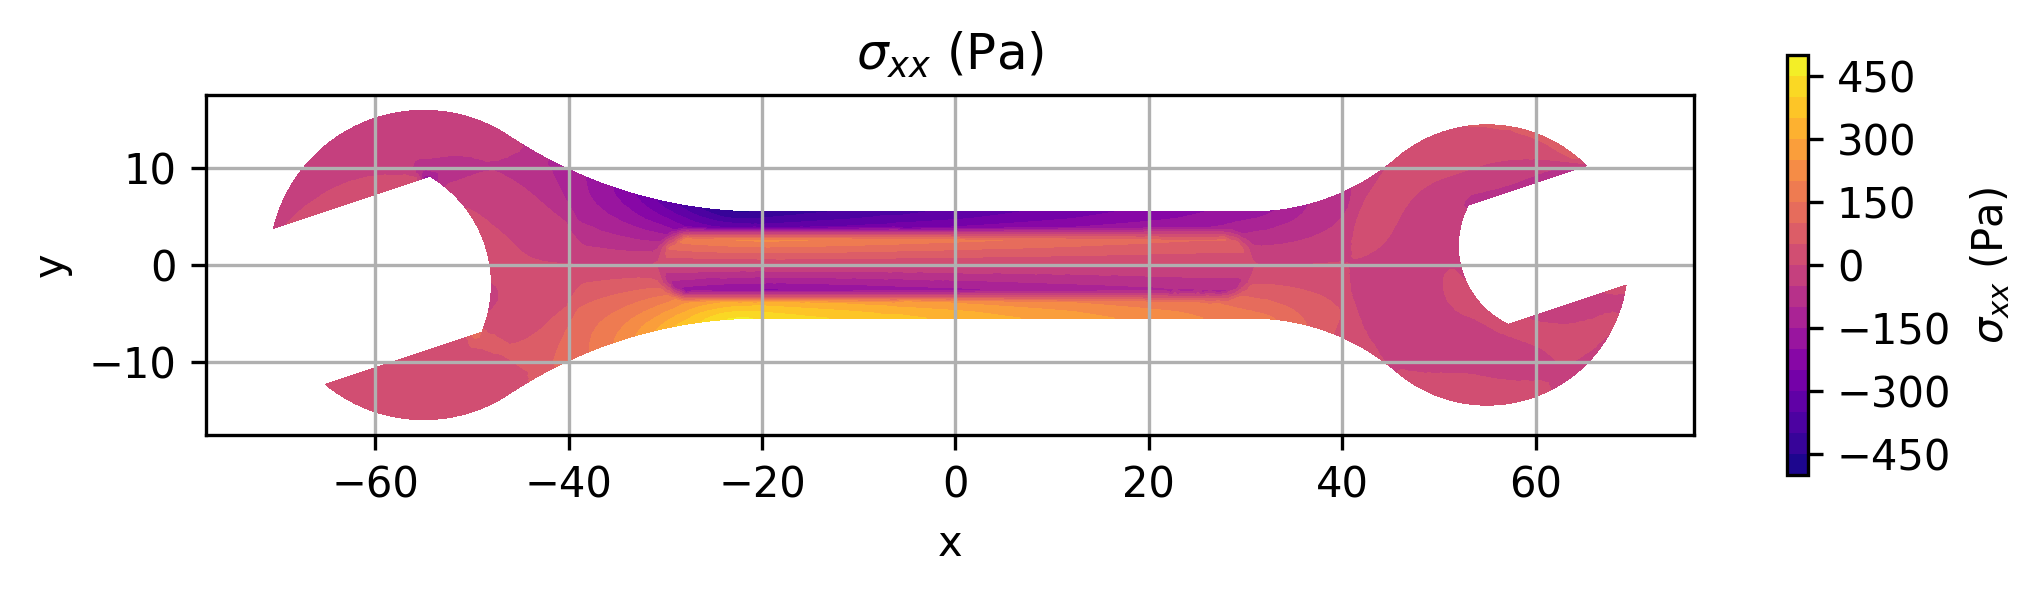
\includegraphics[width=\textwidth]{GRAFICOS/Case a - sigma_xx.png}
    \caption{Caption}
    \label{fig:deformada_reacciones}
  \end{subfigure}
  \hfill
  \begin{subfigure}[t]{0.49\textwidth}
    \centering
    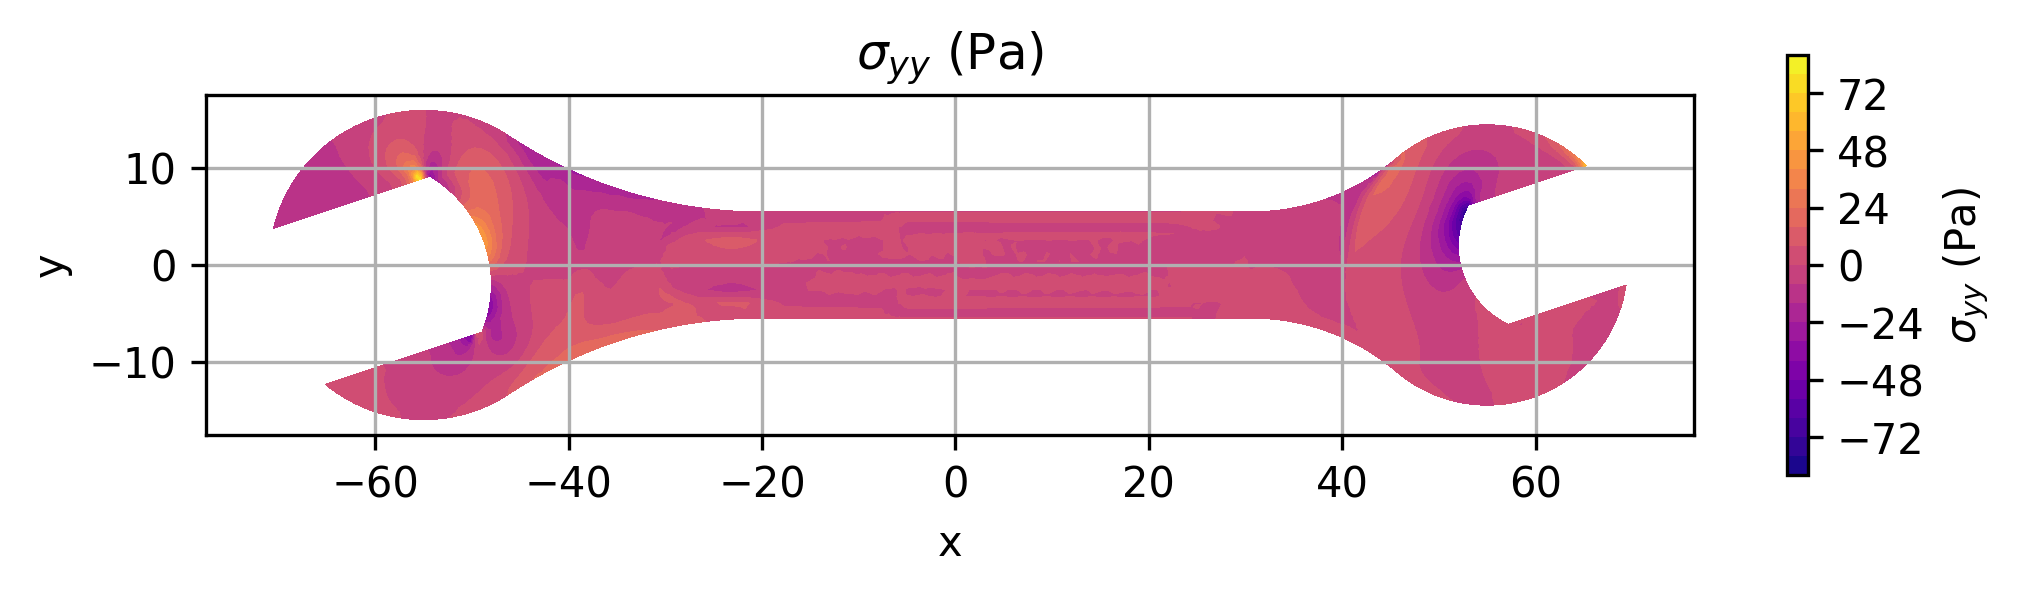
\includegraphics[width=\textwidth]{GRAFICOS/Case a - sigma_yy.png}
    \caption{Caption}
    \label{fig:von_mises}
  \end{subfigure}
  \caption{Caption}
  \label{fig:analisis_estructural}
\end{figure}

\begin{figure}[H]
  \centering
  \begin{subfigure}[t]{0.49\textwidth}
    \centering
    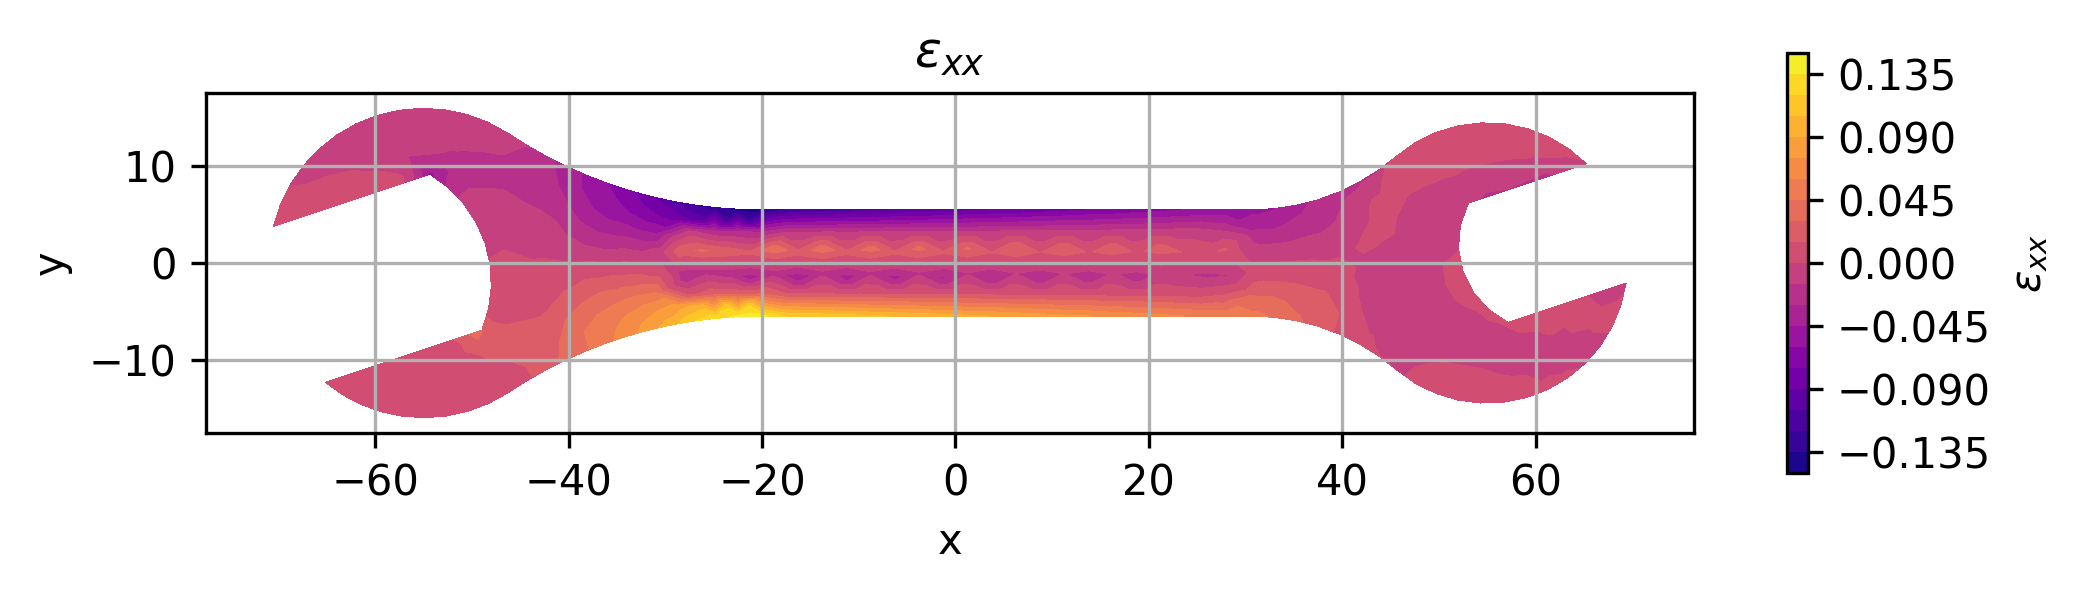
\includegraphics[width=\textwidth]{GRAFICOS/Case a - epsilon_xx.png}
    \caption{Caption}
    \label{fig:deformada_reacciones}
  \end{subfigure}
  \hfill
  \begin{subfigure}[t]{0.49\textwidth}
    \centering
    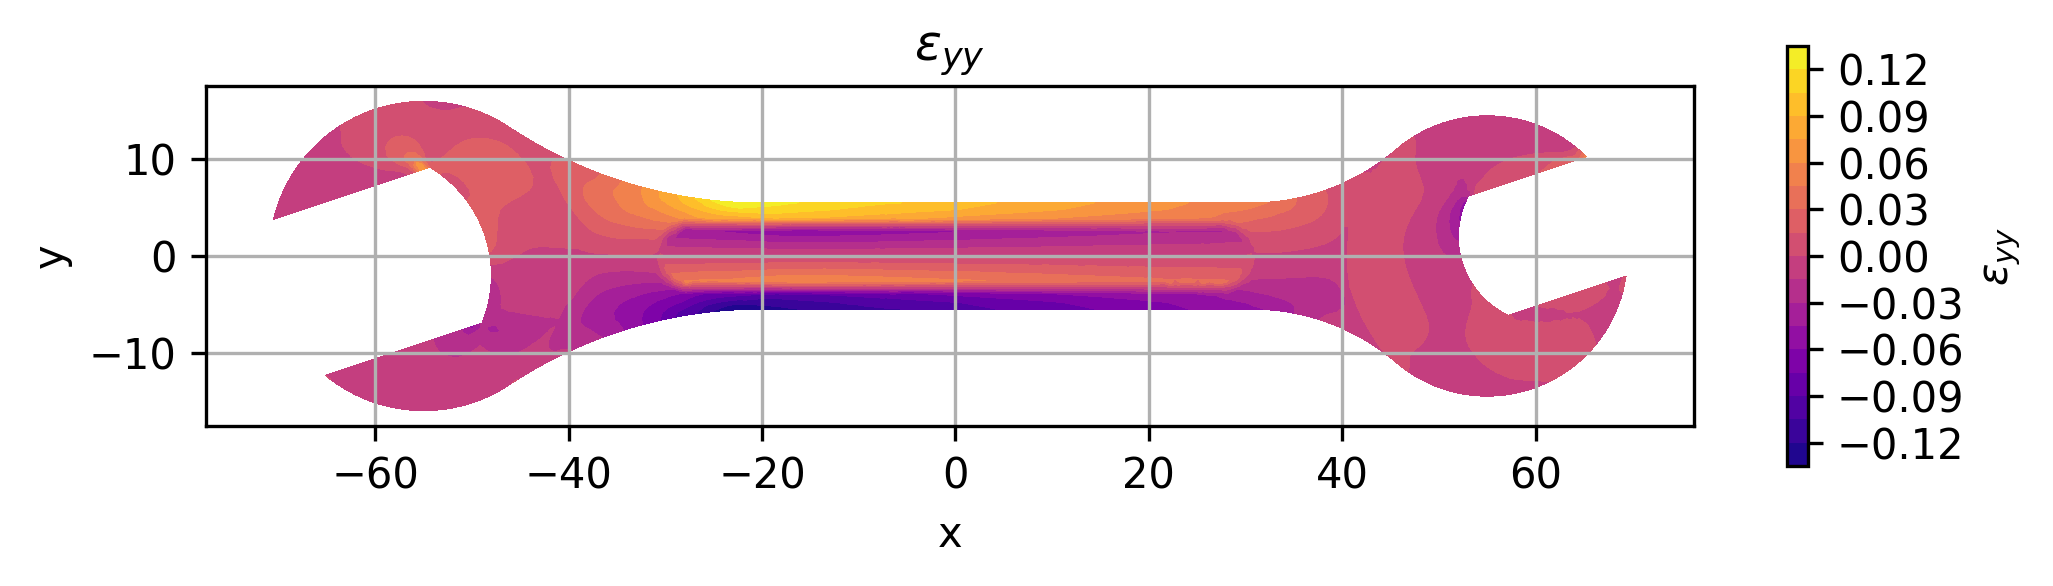
\includegraphics[width=\textwidth]{GRAFICOS/Case a - epsilon_yy.png}
    \caption{Caption}
    \label{fig:von_mises}
  \end{subfigure}
  \caption{Caption}
  \label{fig:analisis_estructural}
\end{figure}

\begin{figure}[H]
  \centering
  \begin{subfigure}[t]{0.49\textwidth}
    \centering
    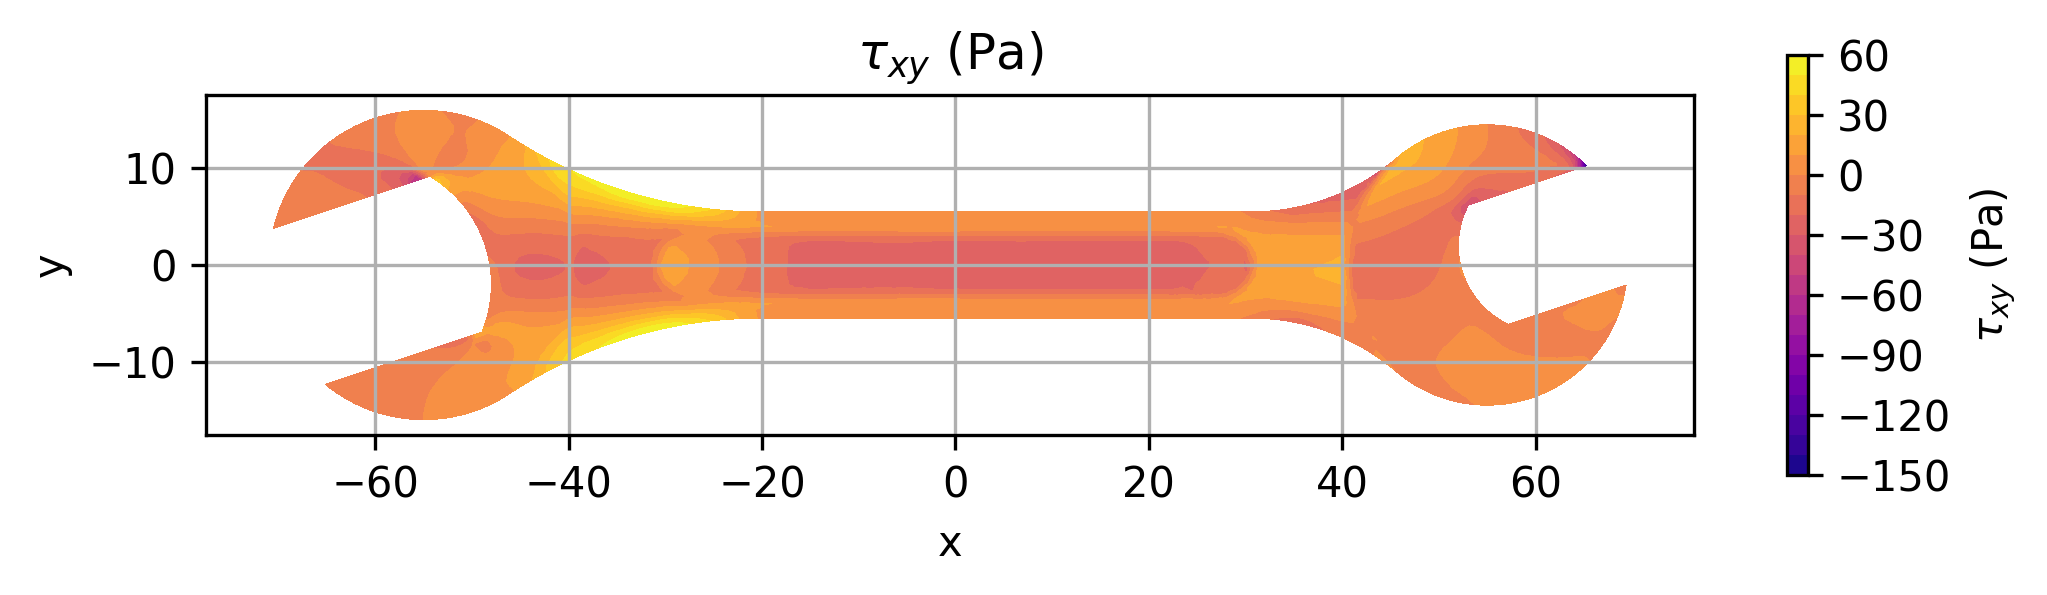
\includegraphics[width=\textwidth]{GRAFICOS/Case a - tau_xy.png}
    \caption{Caption}
    \label{fig:deformada_reacciones}
  \end{subfigure}
  \hfill
  \begin{subfigure}[t]{0.49\textwidth}
    \centering
    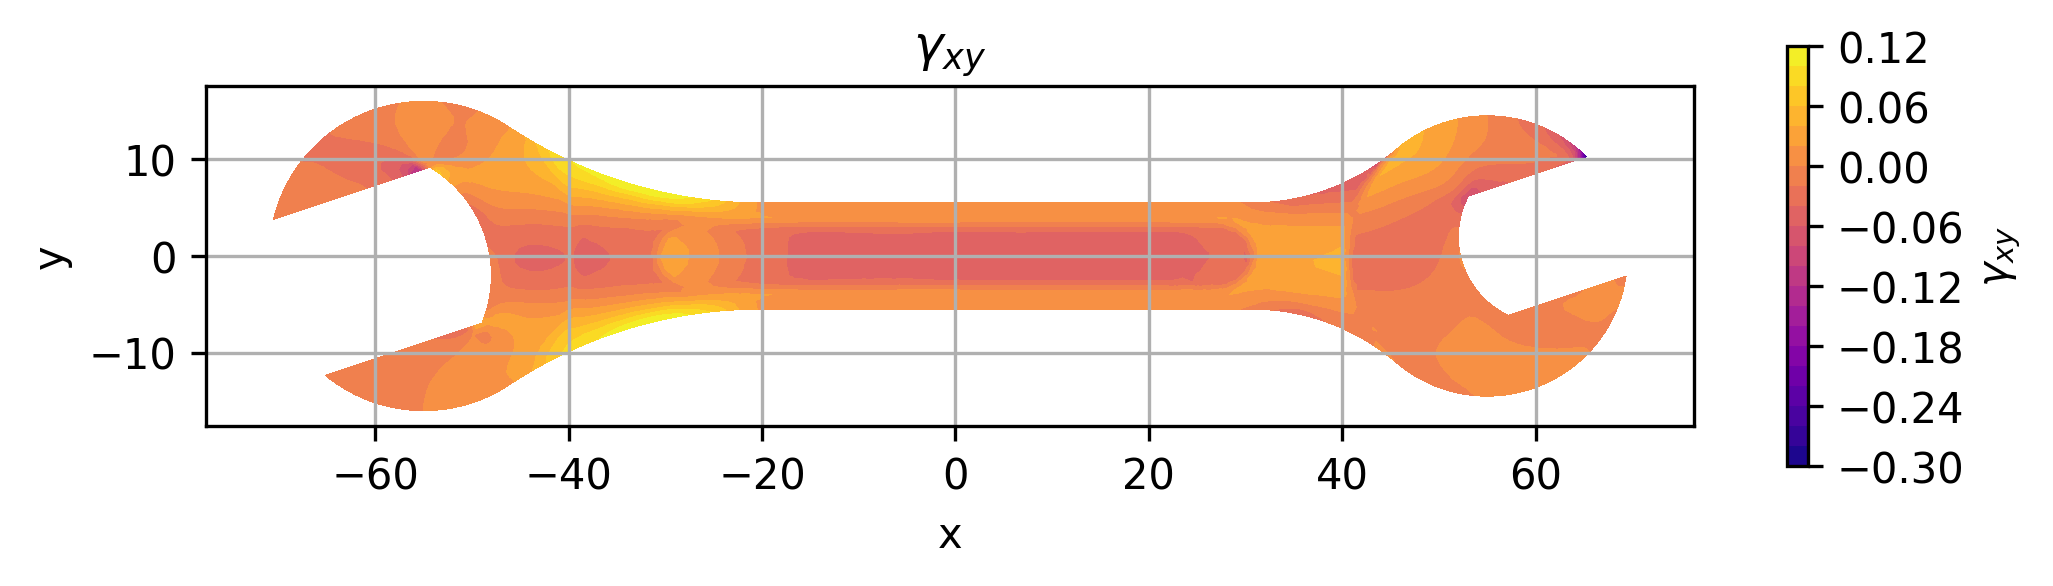
\includegraphics[width=\textwidth]{GRAFICOS/Case a - gamma_xy.png}
    \caption{Caption}
    \label{fig:von_mises}
  \end{subfigure}
  \caption{Caption}
  \label{fig:analisis_estructural}
\end{figure}

\begin{figure}[H]
  \centering
  \begin{subfigure}[t]{0.49\textwidth}
    \centering
    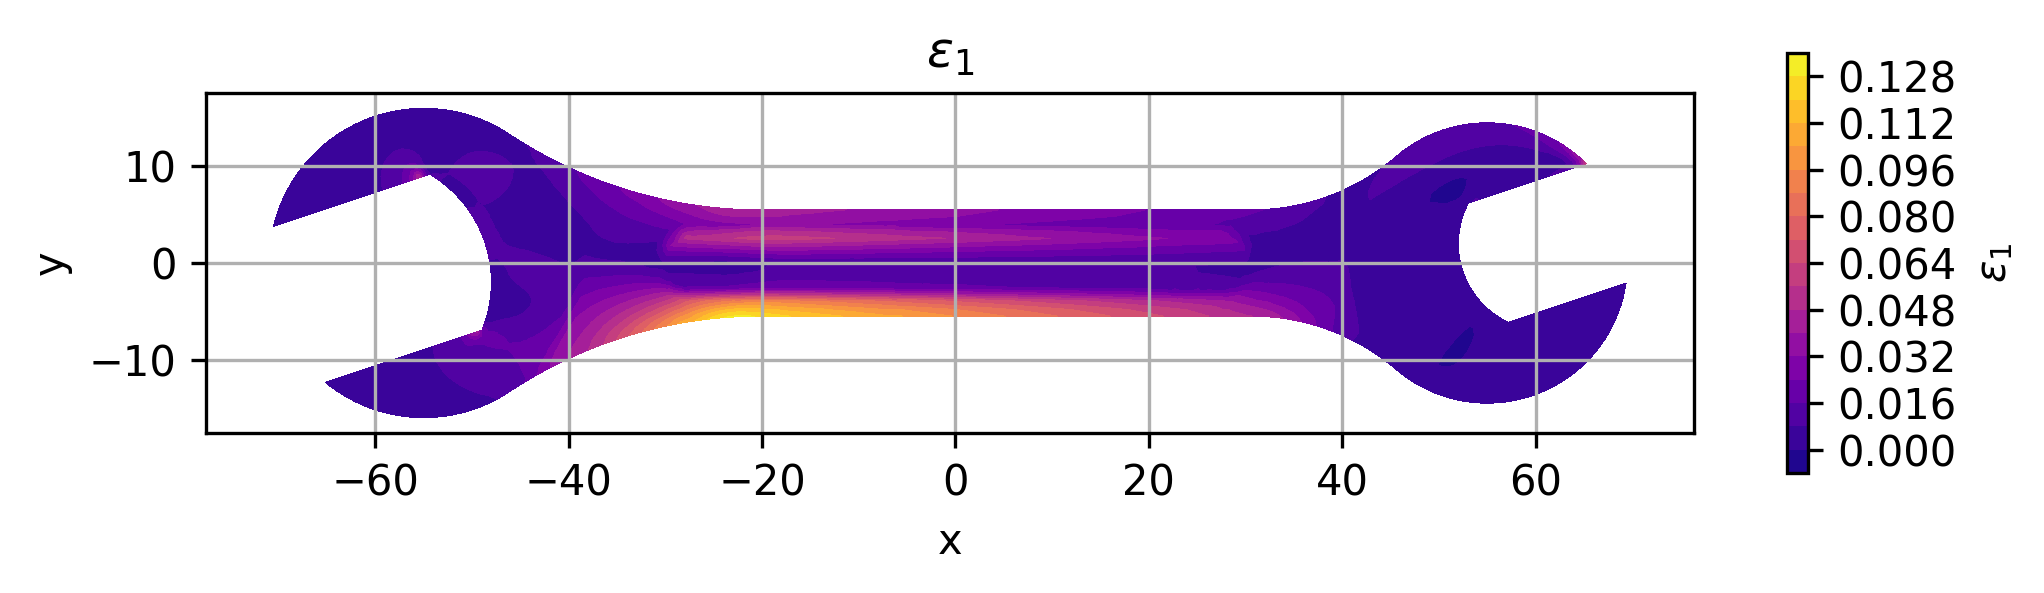
\includegraphics[width=\textwidth]{GRAFICOS/Case a - epsilon_1.png}
    \caption{Caption}
    \label{fig:deformada_reacciones}
  \end{subfigure}
  \hfill
  \begin{subfigure}[t]{0.49\textwidth}
    \centering
    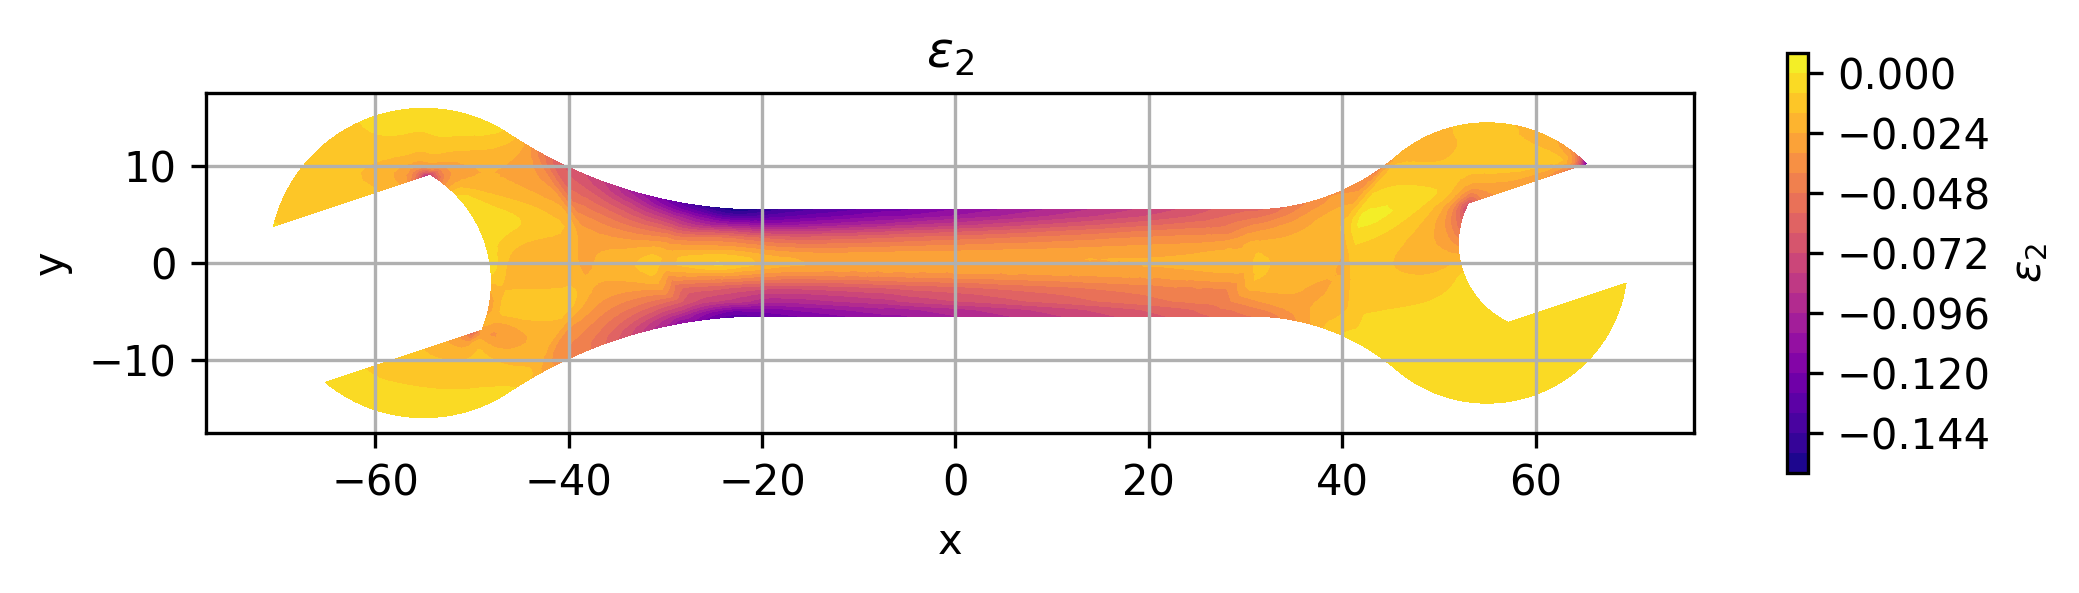
\includegraphics[width=\textwidth]{GRAFICOS/Case a - epsilon_2.png}
    \caption{Caption}
    \label{fig:von_mises}
  \end{subfigure}
  \caption{Caption}
  \label{fig:analisis_estructural}
\end{figure}

\begin{figure}[H]
  \centering
  \begin{subfigure}[t]{0.49\textwidth}
    \centering
    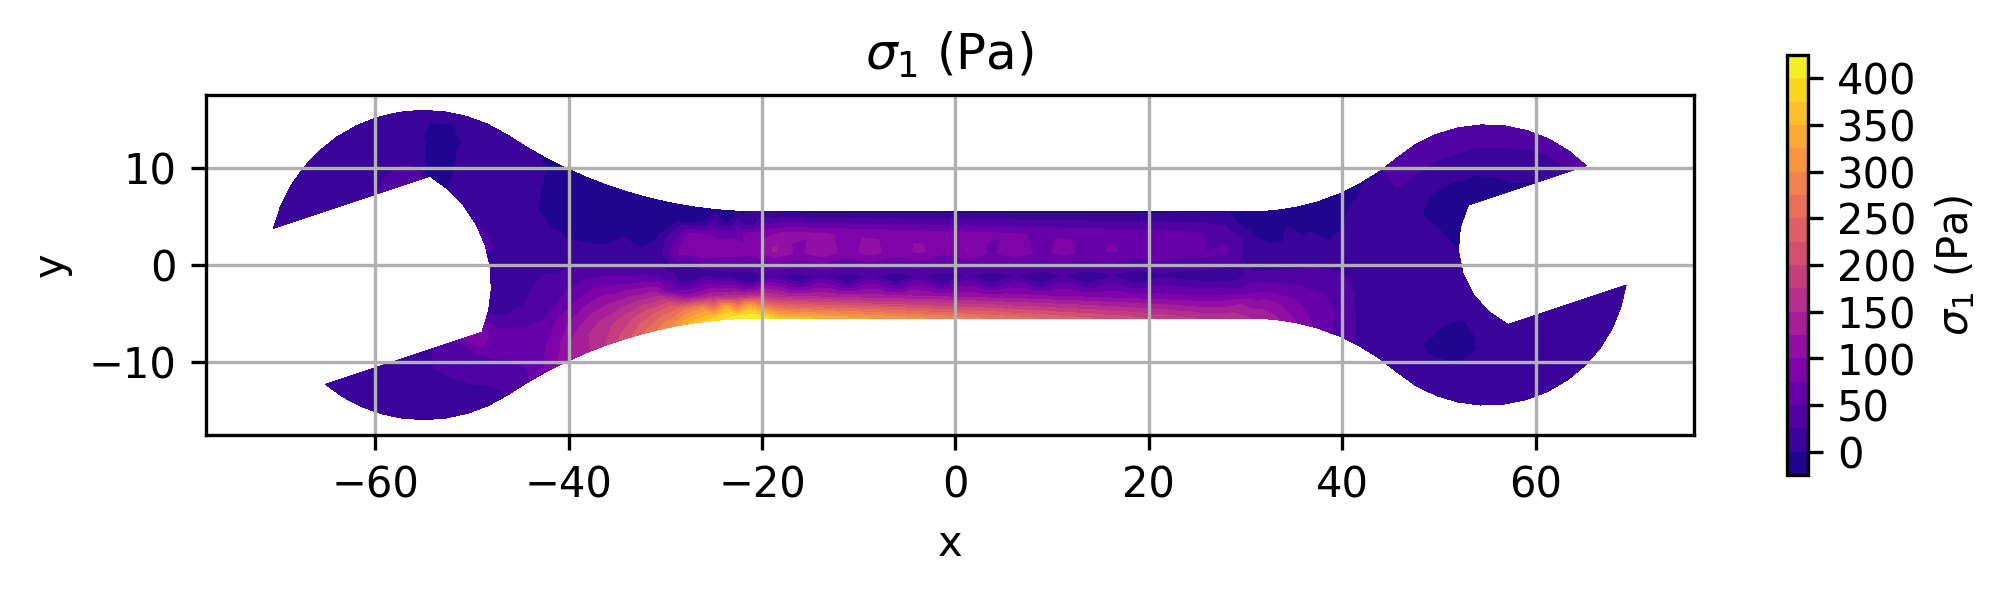
\includegraphics[width=\textwidth]{GRAFICOS/Case a - sigma_1.png}
    \caption{Caption}
    \label{fig:deformada_reacciones}
  \end{subfigure}
  \hfill
  \begin{subfigure}[t]{0.49\textwidth}
    \centering
    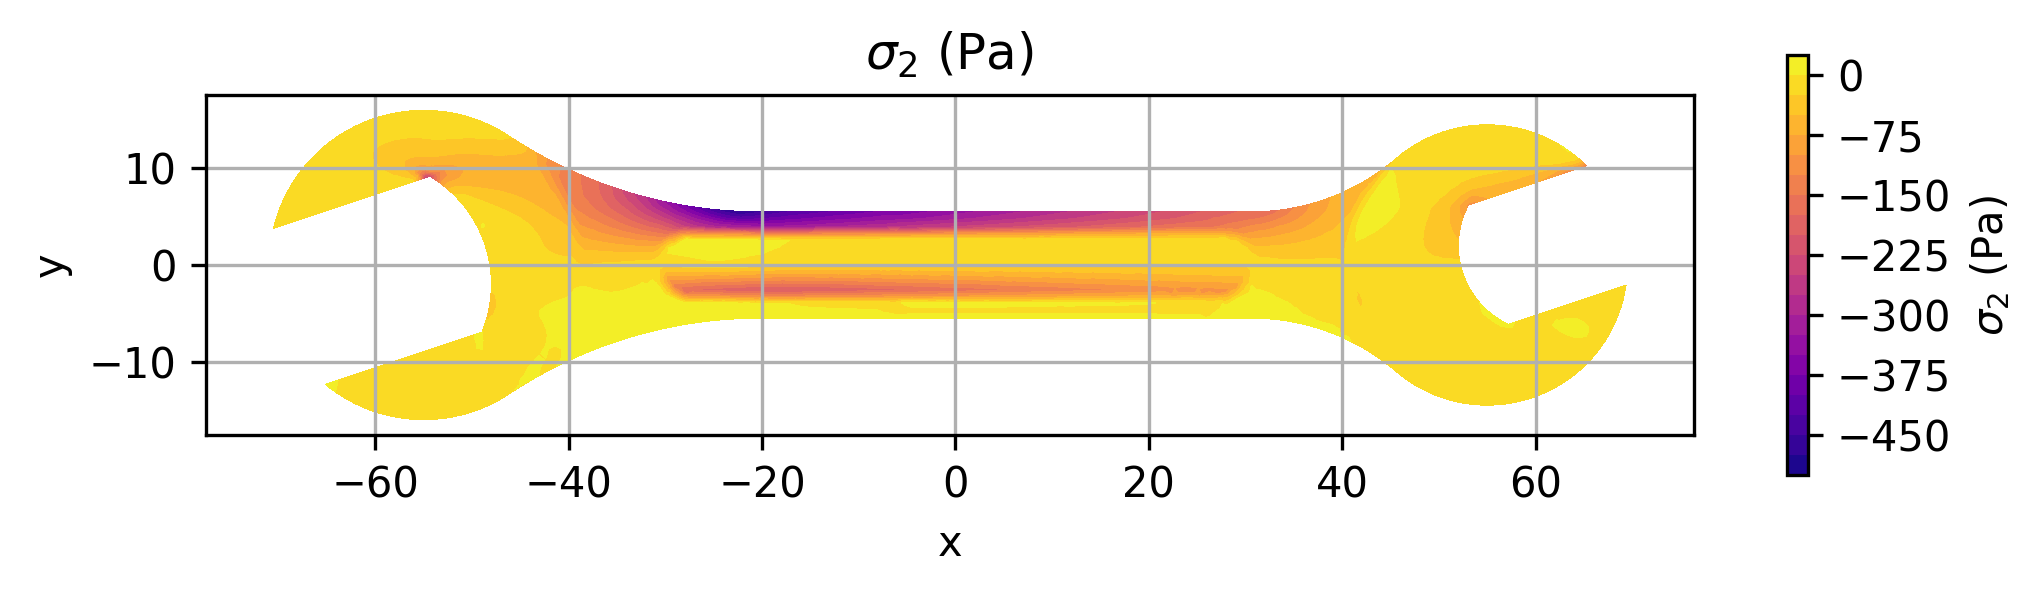
\includegraphics[width=\textwidth]{GRAFICOS/Case a - sigma_2.png}
    \caption{Caption}
    \label{fig:von_mises}
  \end{subfigure}
  \caption{Caption}
  \label{fig:analisis_estructural}
\end{figure}



\section{B case}

\begin{figure}[H]
  \centering
  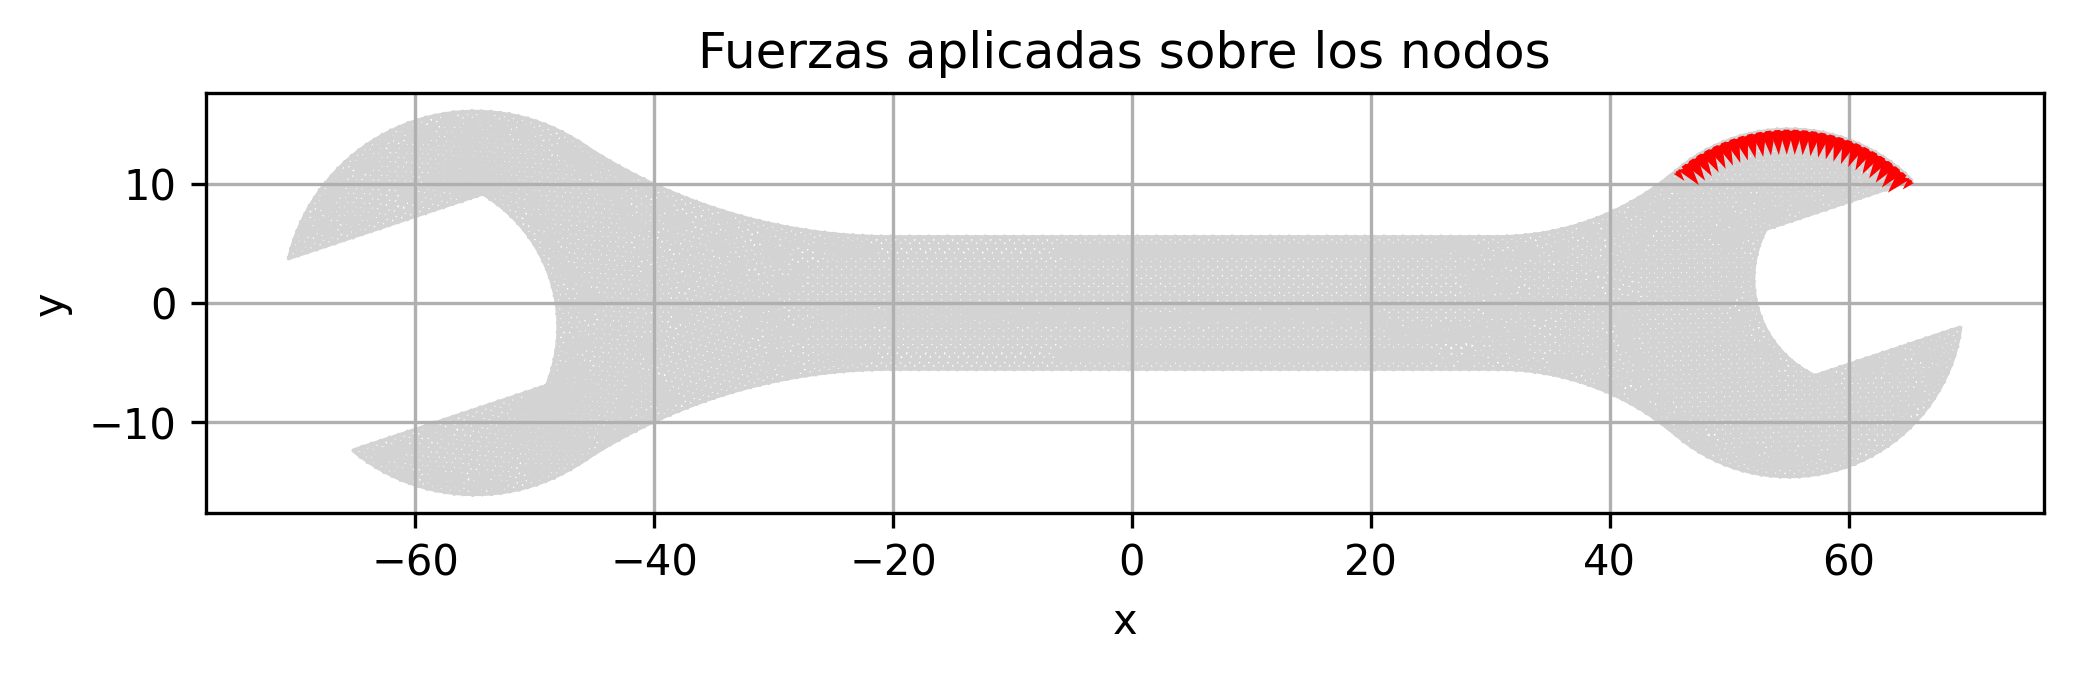
\includegraphics[width=0.8\textwidth]{GRAFICOS/Case b_fuerzas.png}
  \caption{Caption}
  \label{fig:strain}
\end{figure}

\begin{figure}[H]
  \centering
  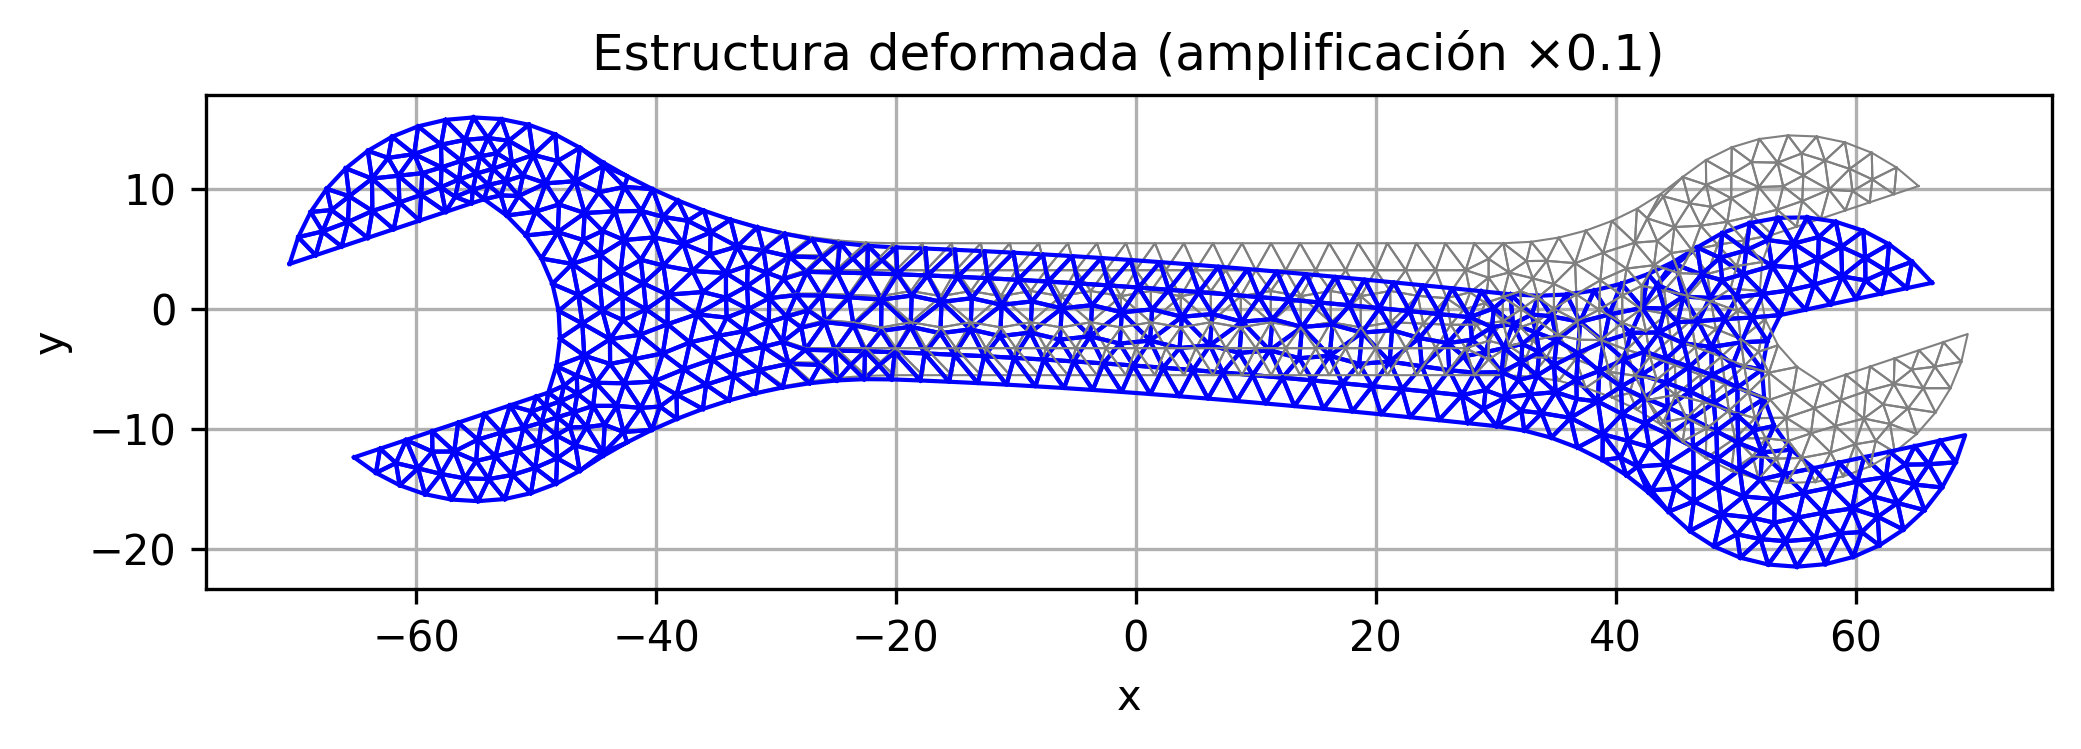
\includegraphics[width=0.8\textwidth]{GRAFICOS/Case b_deformada.png}
  \caption{Caption}
  \label{fig:stress}
\end{figure}

\begin{figure}[H]
  \centering
  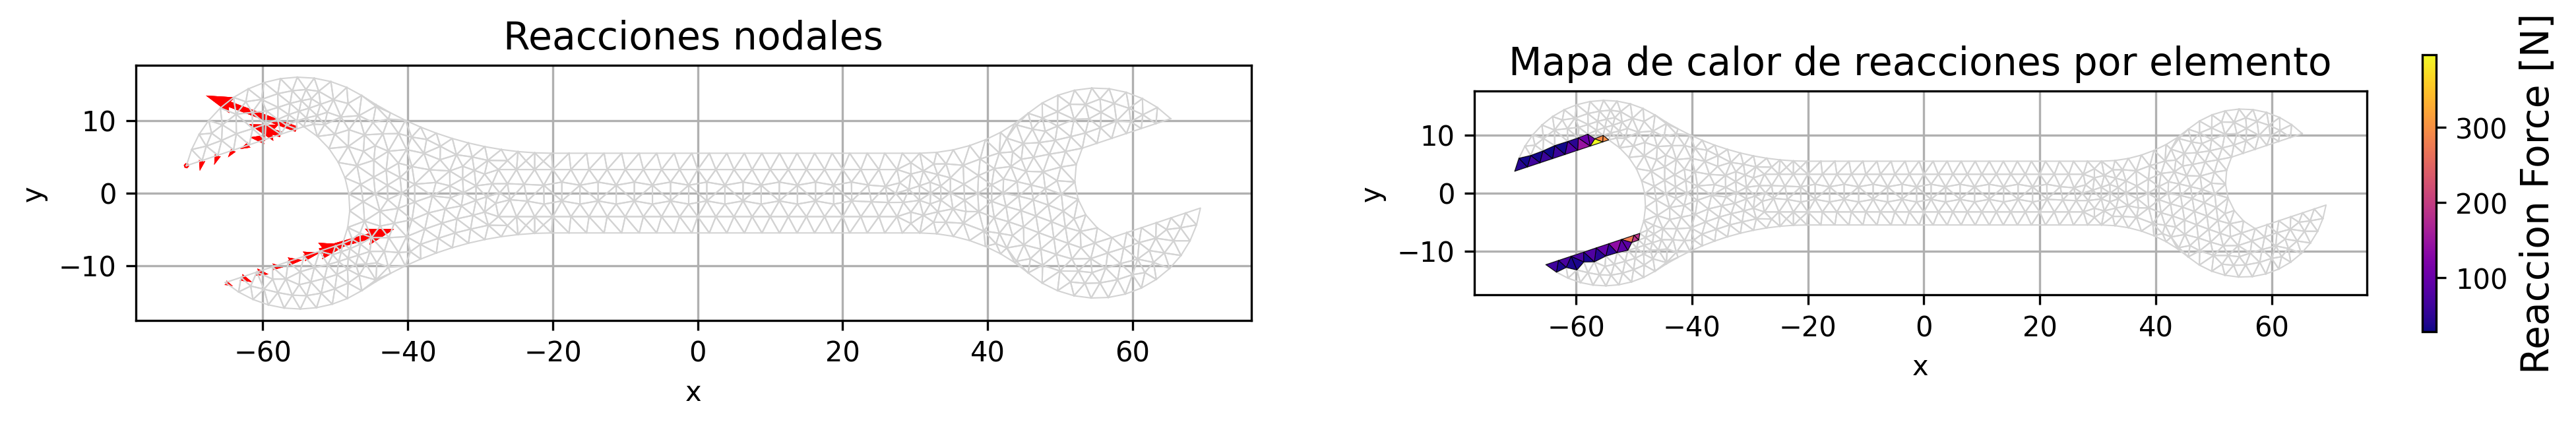
\includegraphics[width=1\textwidth]{GRAFICOS/Case b_deformada_reacciones.png}
  \caption{Caption}
  \label{fig:principal}
\end{figure}

\begin{figure}[H]
  \centering
  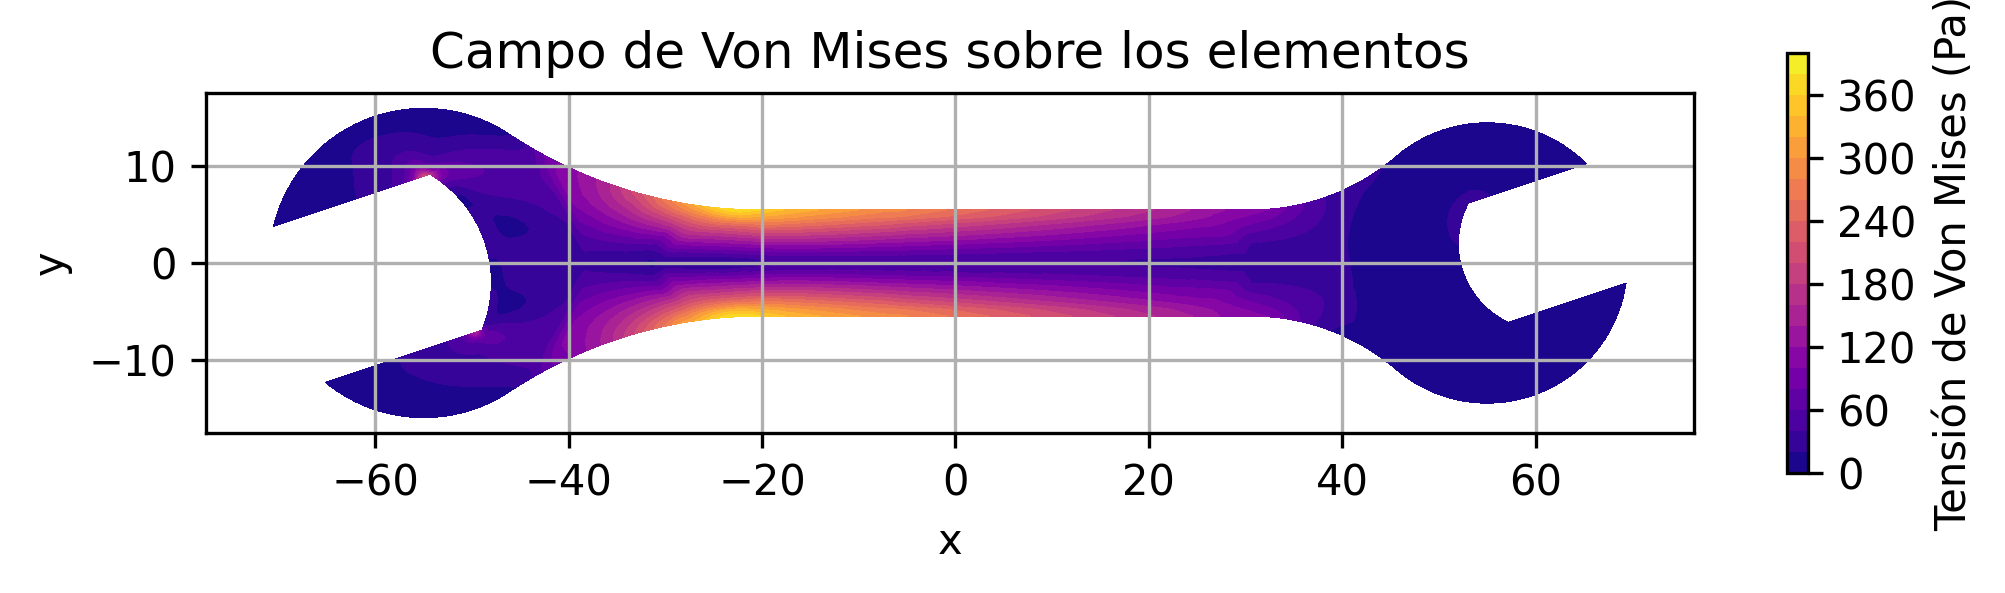
\includegraphics[width=0.8\textwidth]{GRAFICOS/Case b_von_mises.png}
  \caption{Caption}
  \label{fig:principal}
\end{figure}

\begin{figure}[H]
  \centering
  \begin{subfigure}[t]{0.49\textwidth}
    \centering
    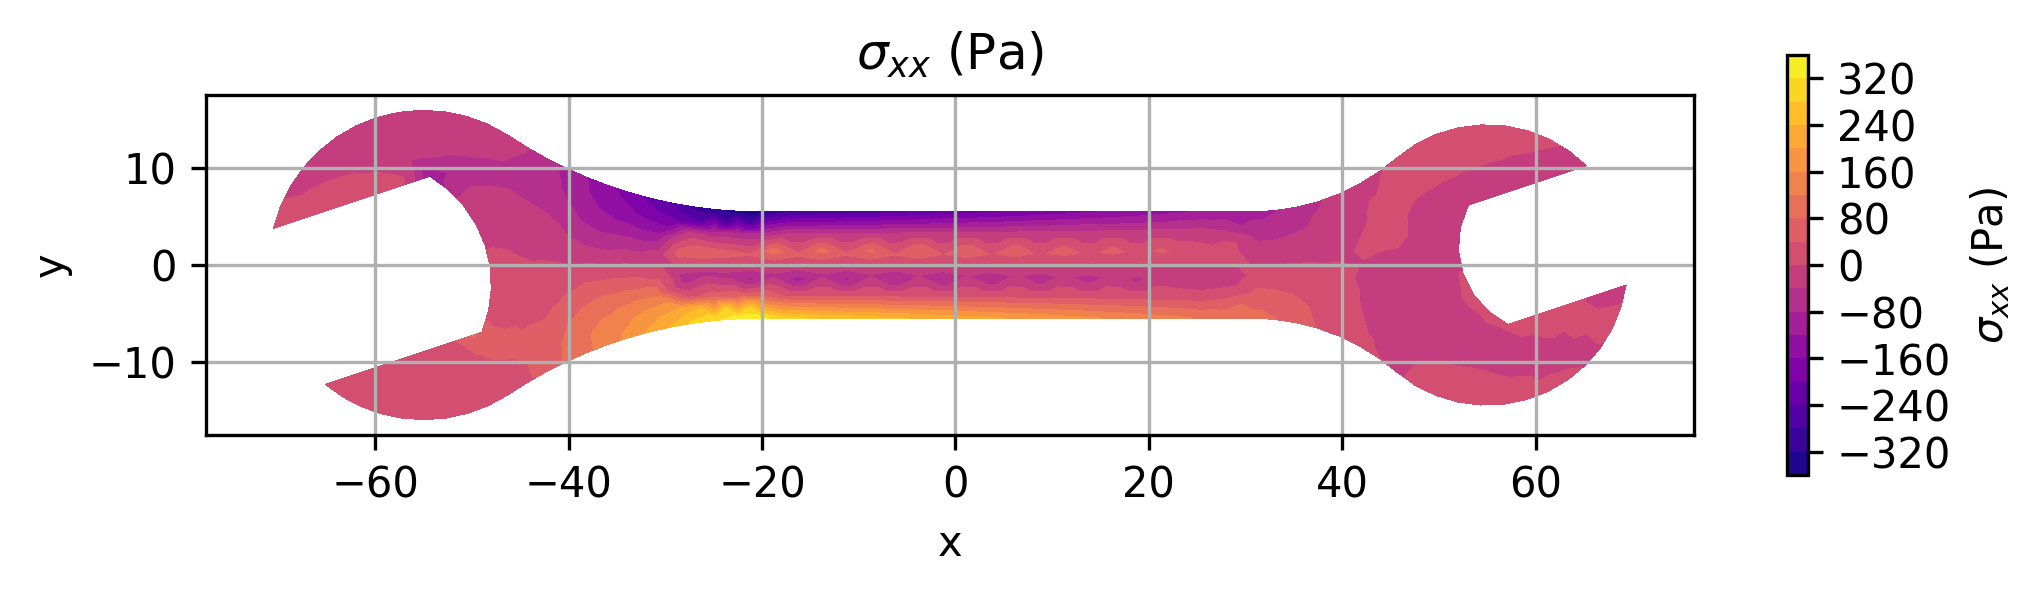
\includegraphics[width=\textwidth]{GRAFICOS/Case b - sigma_xx.png}
    \caption{Caption}
    \label{fig:deformada_reacciones}
  \end{subfigure}
  \hfill
  \begin{subfigure}[t]{0.49\textwidth}
    \centering
    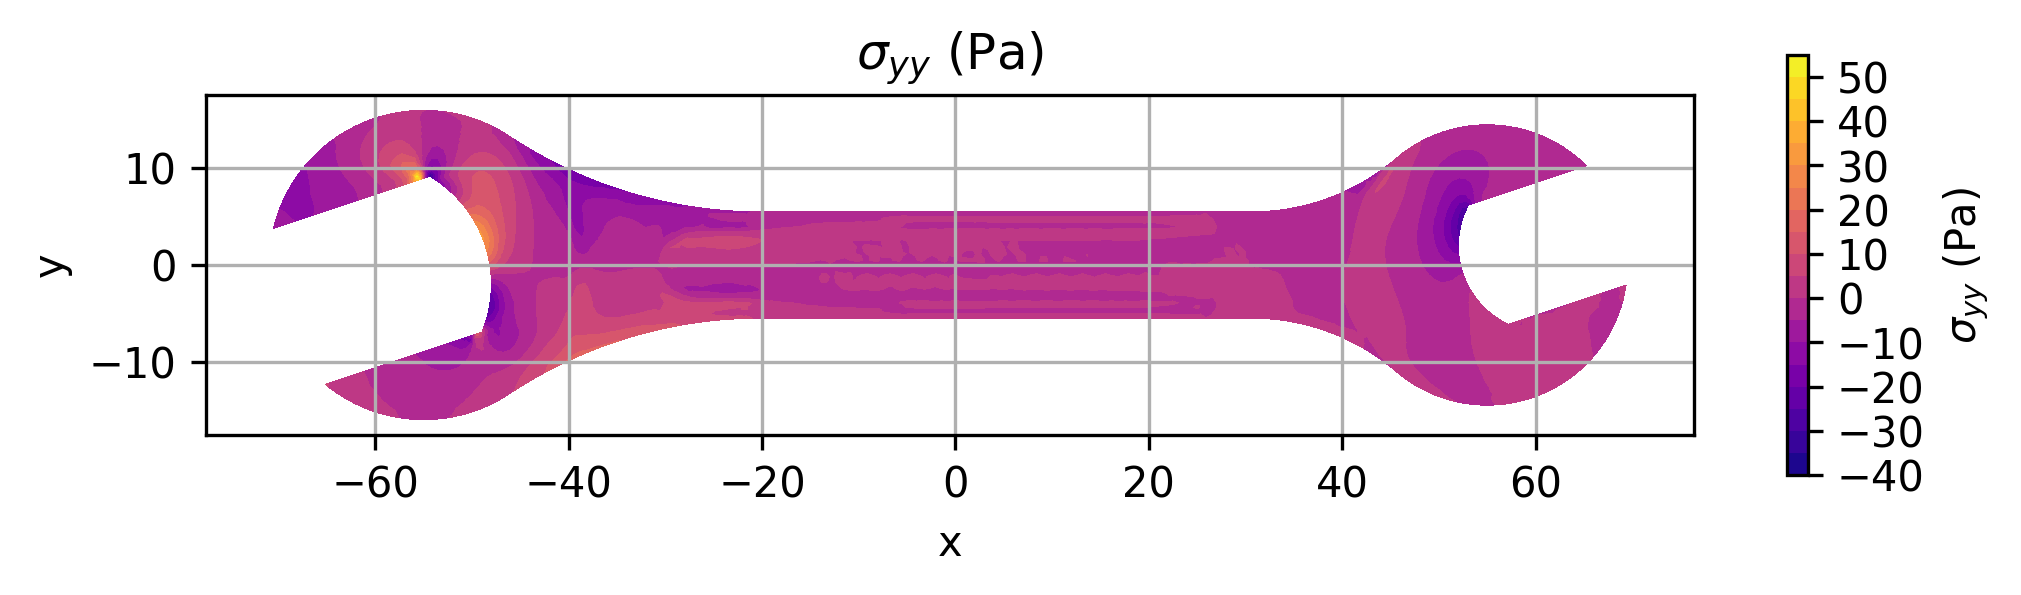
\includegraphics[width=\textwidth]{GRAFICOS/Case b - sigma_yy.png}
    \caption{Caption}
    \label{fig:von_mises}
  \end{subfigure}
  \caption{Caption}
  \label{fig:analisis_estructural}
\end{figure}

\begin{figure}[H]
  \centering
  \begin{subfigure}[t]{0.49\textwidth}
    \centering
    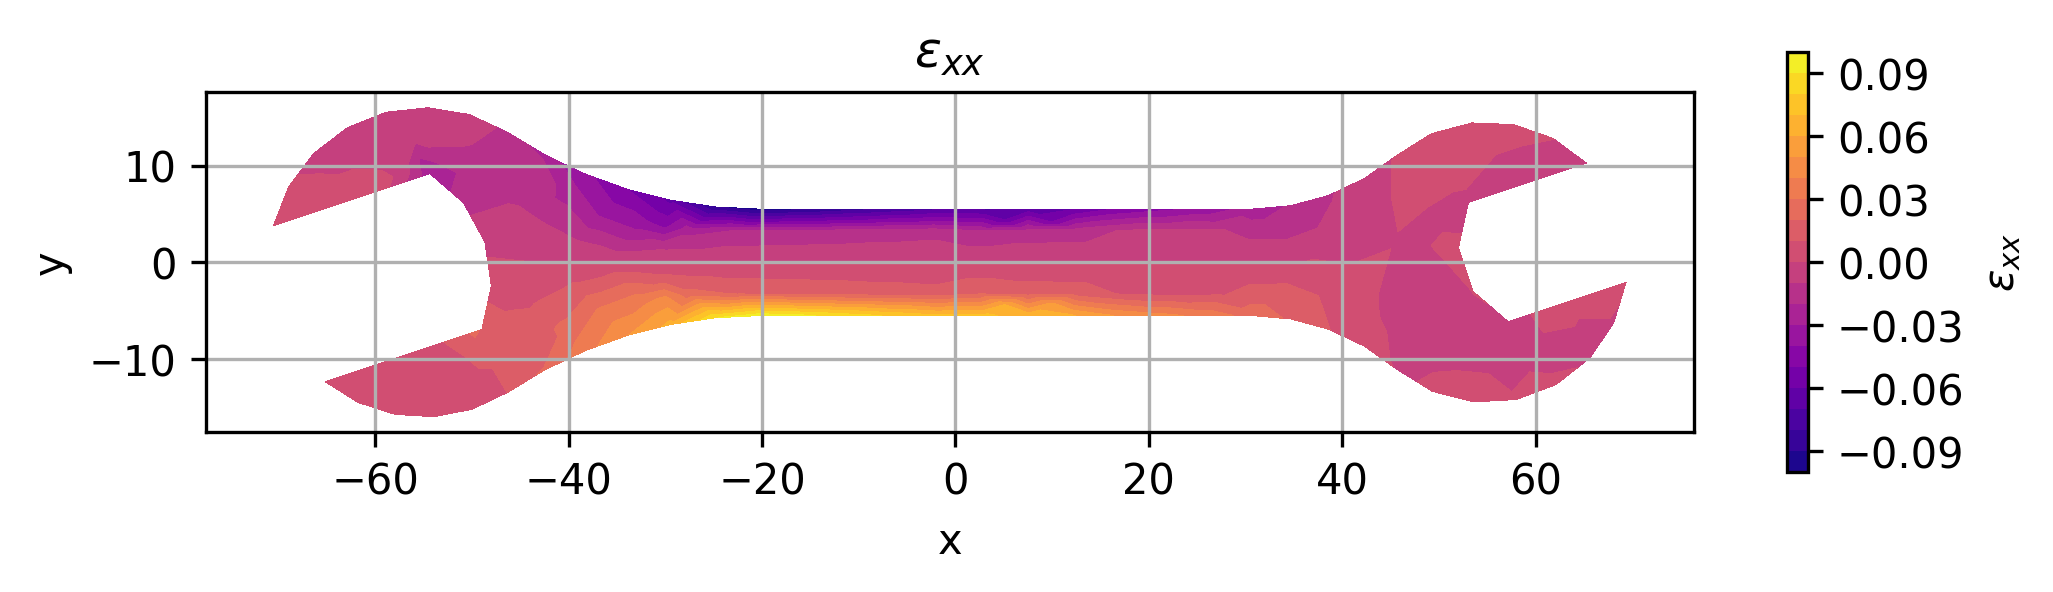
\includegraphics[width=\textwidth]{GRAFICOS/Case b - epsilon_xx.png}
    \caption{Caption}
    \label{fig:deformada_reacciones}
  \end{subfigure}
  \hfill
  \begin{subfigure}[t]{0.49\textwidth}
    \centering
    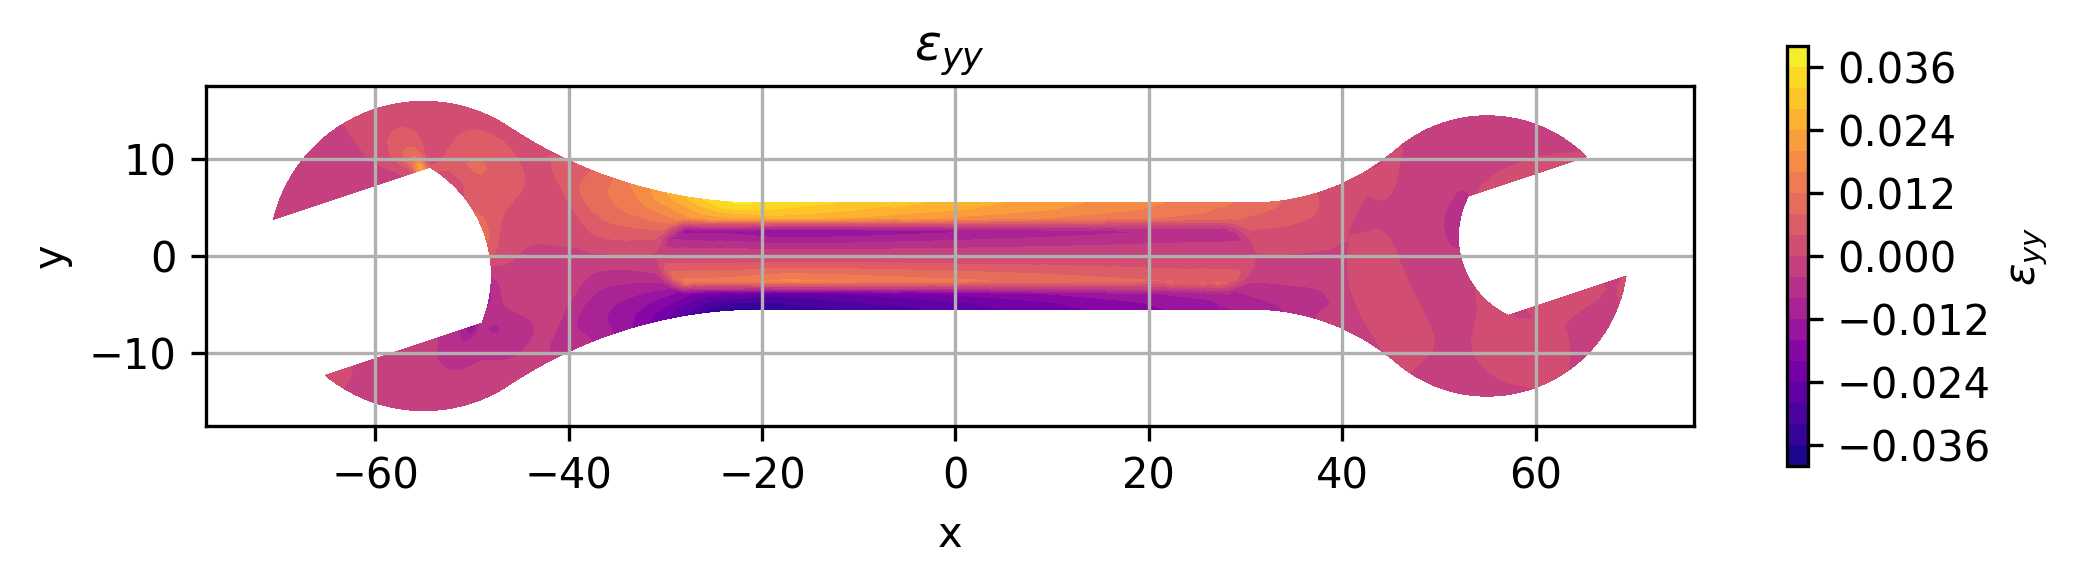
\includegraphics[width=\textwidth]{GRAFICOS/Case b - epsilon_yy.png}
    \caption{Caption}
    \label{fig:von_mises}
  \end{subfigure}
  \caption{Caption}
  \label{fig:analisis_estructural}
\end{figure}


\begin{figure}[H]
  \centering
  \begin{subfigure}[t]{0.49\textwidth}
    \centering
    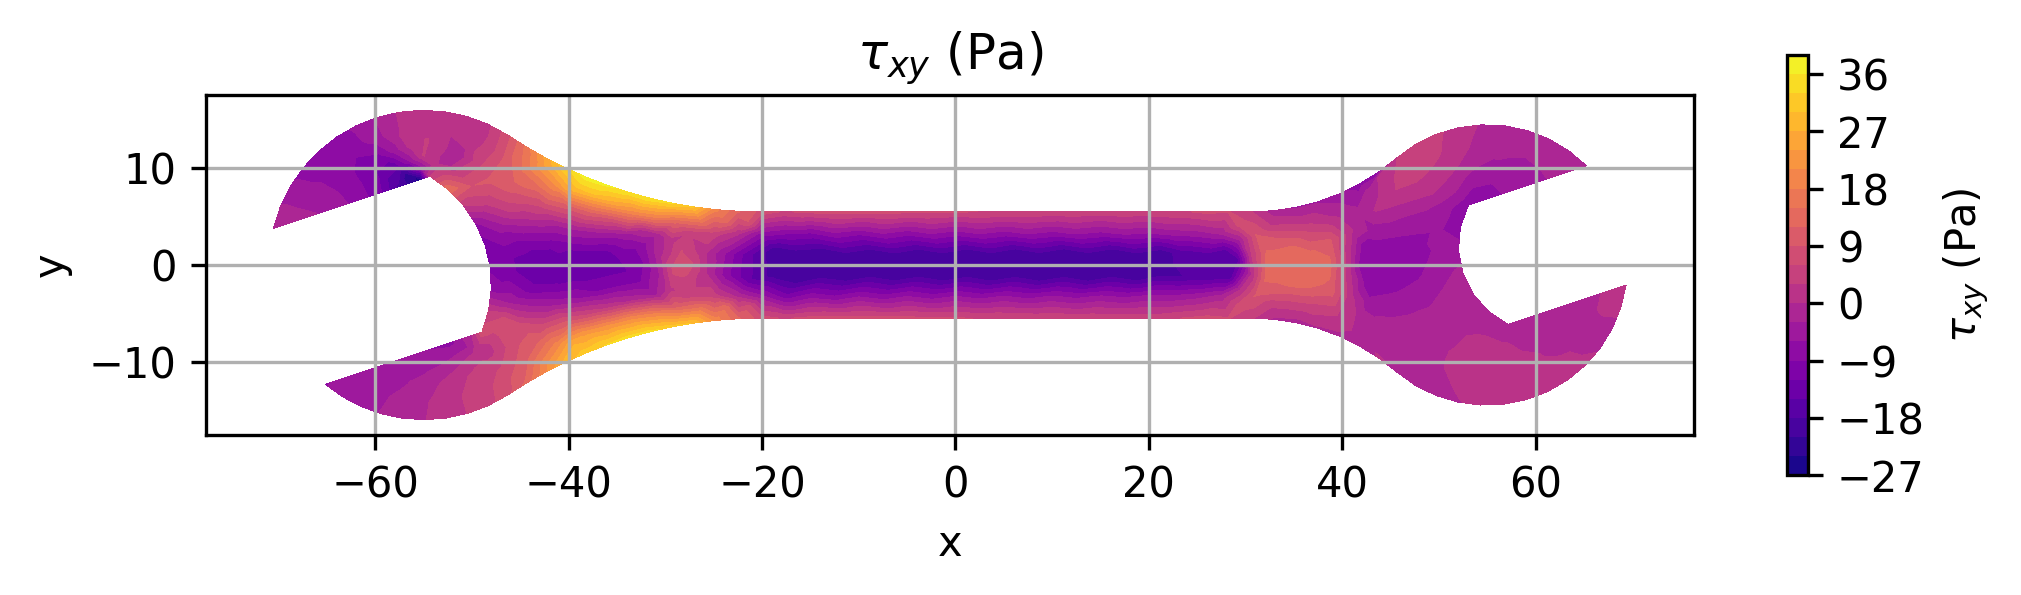
\includegraphics[width=\textwidth]{GRAFICOS/Case b - tau_xy.png}
    \caption{Caption}
    \label{fig:deformada_reacciones}
  \end{subfigure}
  \hfill
  \begin{subfigure}[t]{0.49\textwidth}
    \centering
    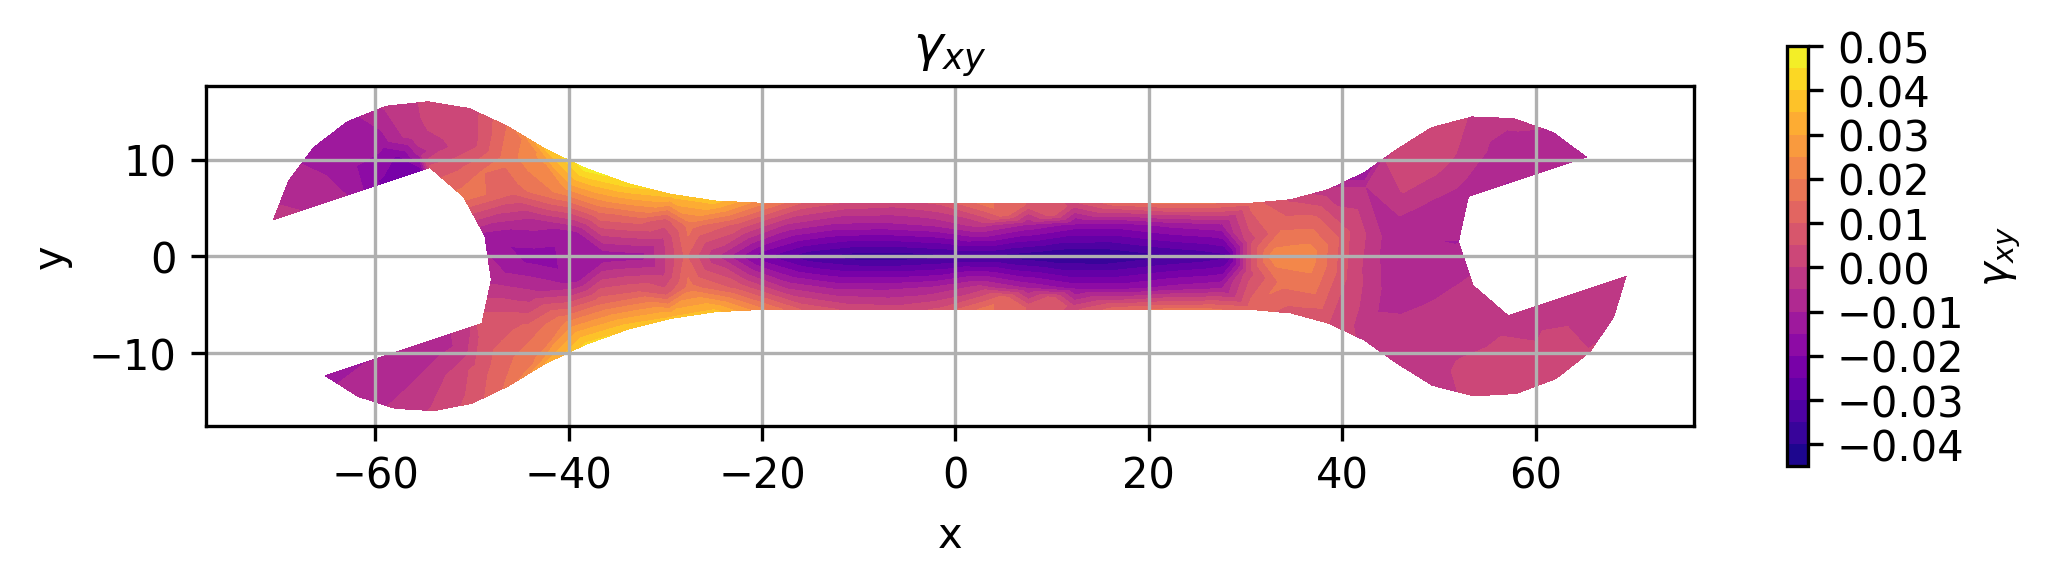
\includegraphics[width=\textwidth]{GRAFICOS/Case b - gamma_xy.png}
    \caption{Caption}
    \label{fig:von_mises}
  \end{subfigure}
  \caption{Caption}
  \label{fig:analisis_estructural}
\end{figure}

\begin{figure}[H]
  \centering
  \begin{subfigure}[t]{0.49\textwidth}
    \centering
    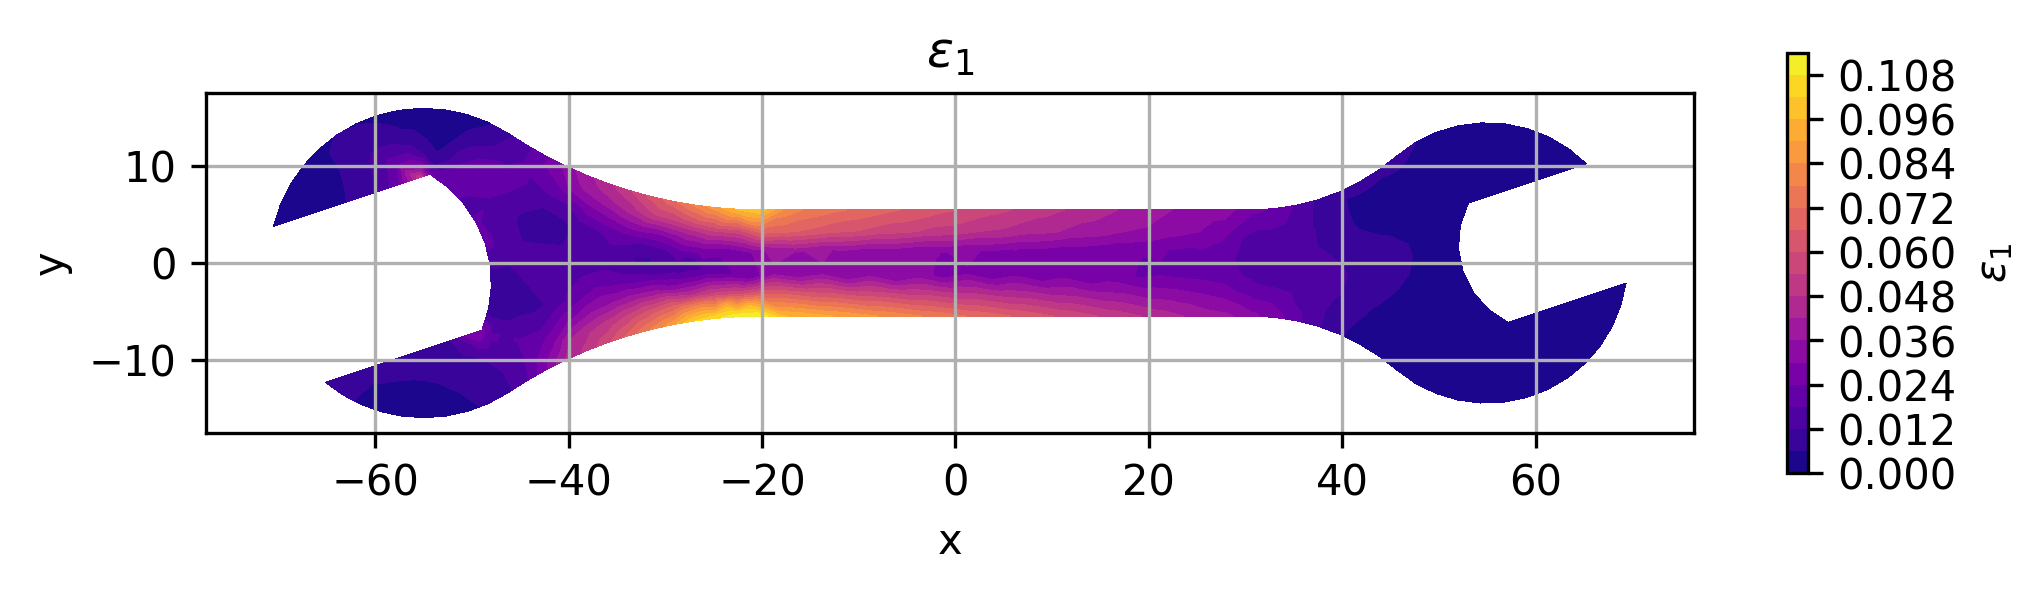
\includegraphics[width=\textwidth]{GRAFICOS/Case b - epsilon_1.png}
    \caption{Caption}
    \label{fig:deformada_reacciones}
  \end{subfigure}
  \hfill
  \begin{subfigure}[t]{0.49\textwidth}
    \centering
    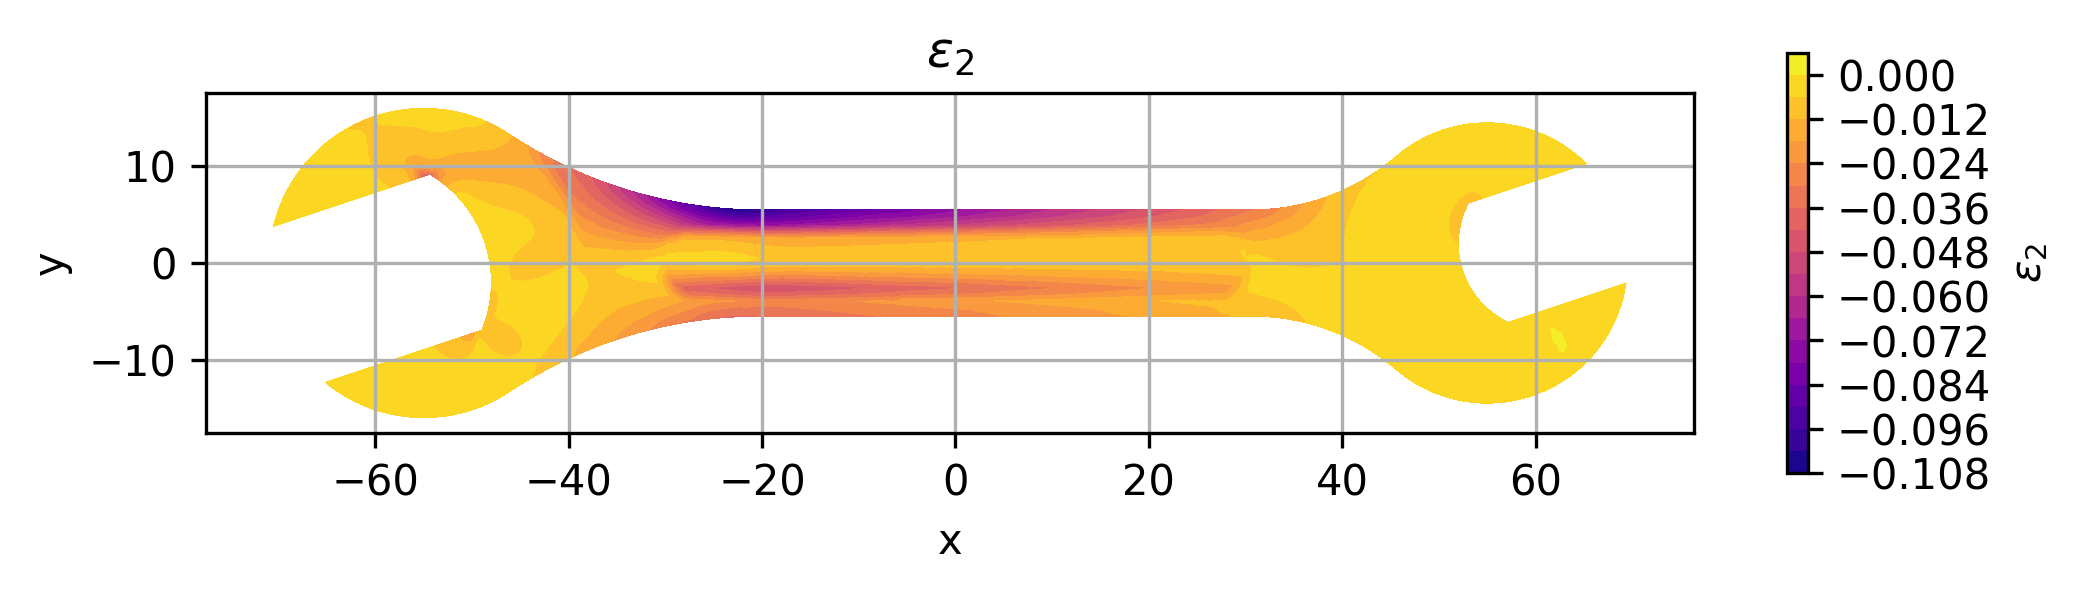
\includegraphics[width=\textwidth]{GRAFICOS/Case b - epsilon_2.png}
    \caption{Caption}
    \label{fig:von_mises}
  \end{subfigure}
  \caption{Caption}
  \label{fig:analisis_estructural}
\end{figure}

\begin{figure}[H]
  \centering
  \begin{subfigure}[t]{0.49\textwidth}
    \centering
    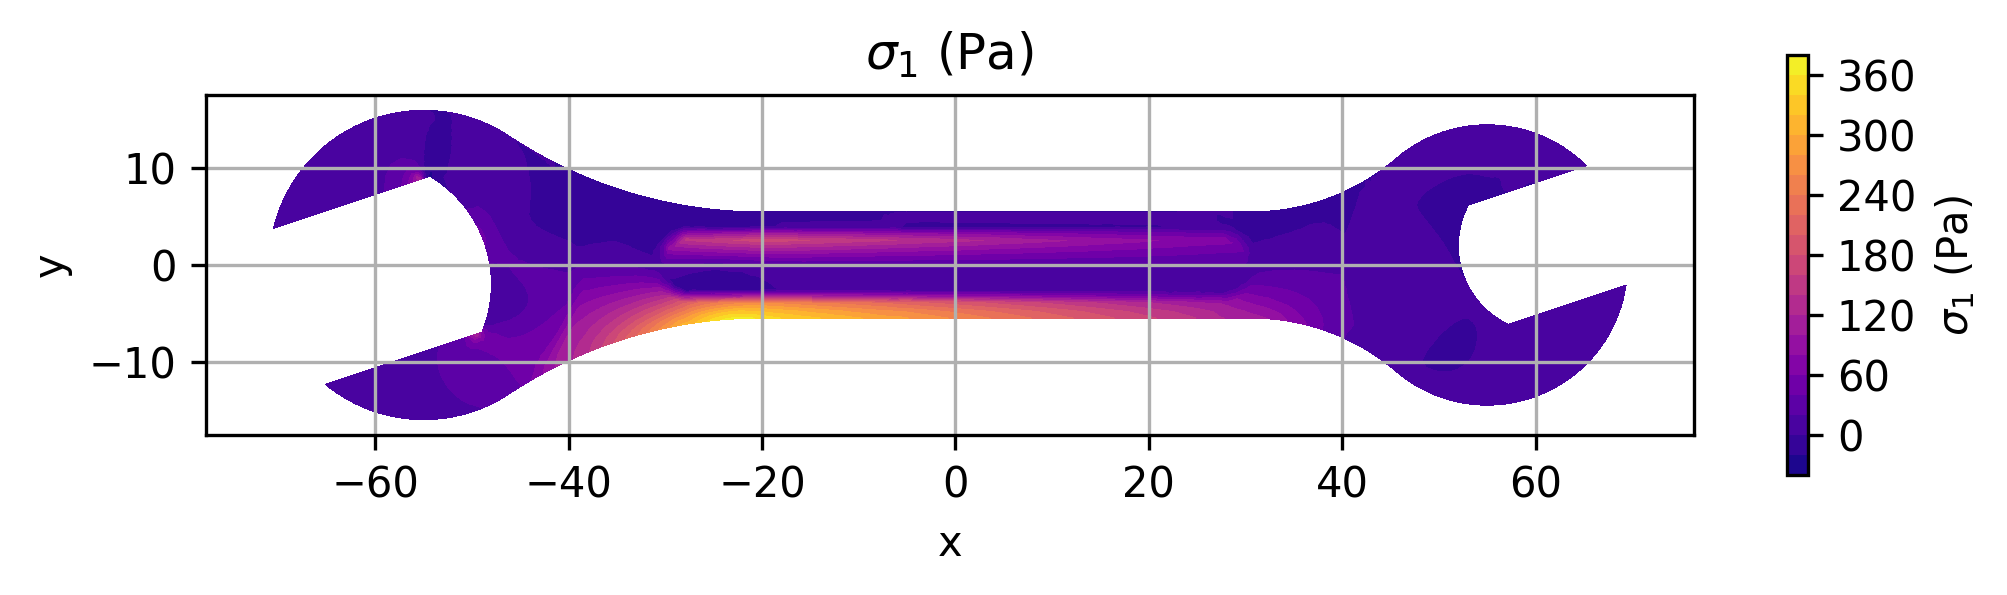
\includegraphics[width=\textwidth]{GRAFICOS/Case b - sigma_1.png}
    \caption{Caption}
    \label{fig:deformada_reacciones}
  \end{subfigure}
  \hfill
  \begin{subfigure}[t]{0.49\textwidth}
    \centering
    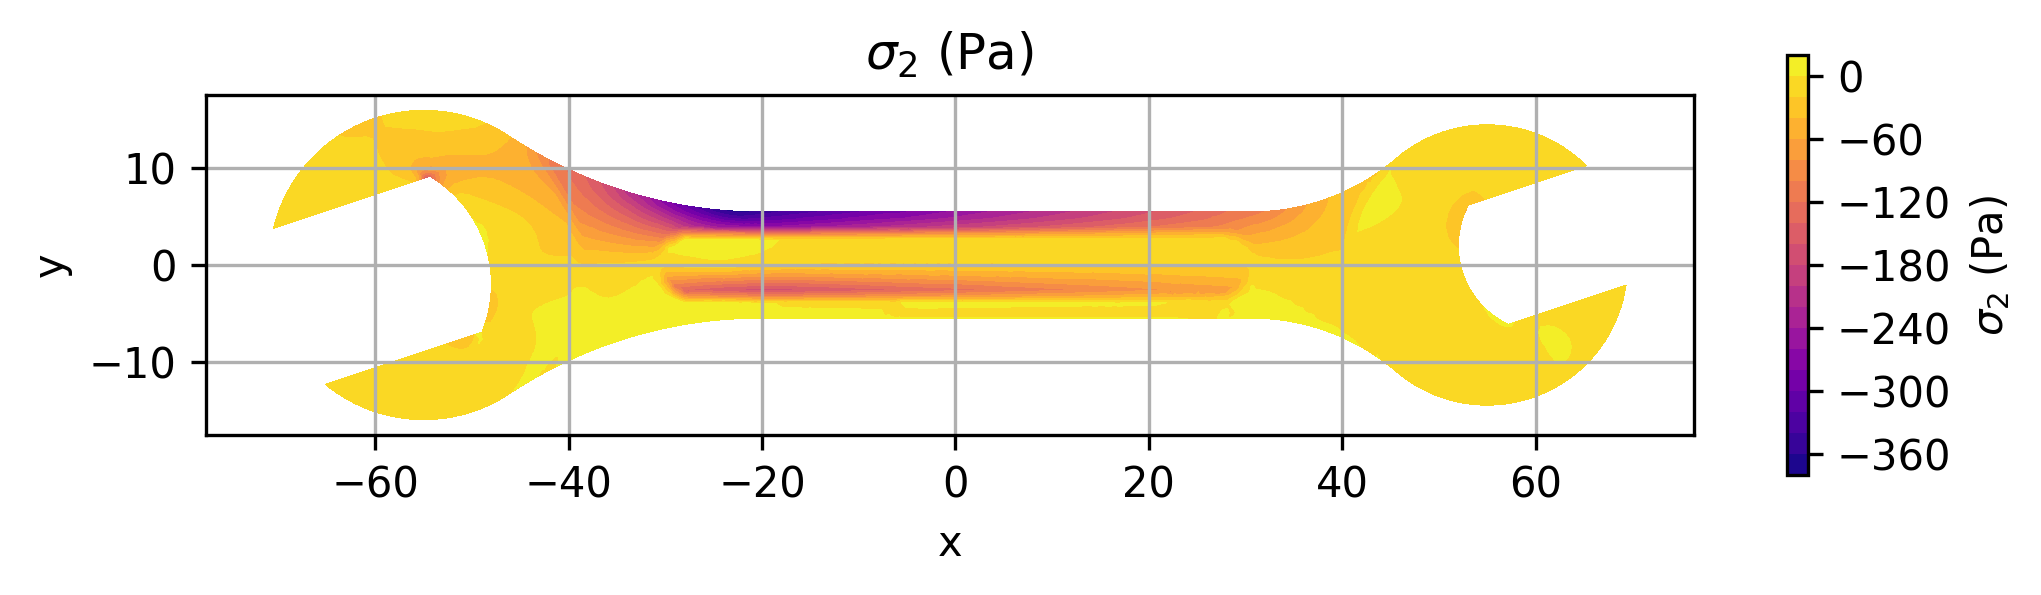
\includegraphics[width=\textwidth]{GRAFICOS/Case b - sigma_2.png}
    \caption{Caption}
    \label{fig:von_mises}
  \end{subfigure}
  \caption{Caption}
  \label{fig:analisis_estructural}
\end{figure}

\section{C case}

\begin{figure}[H]
  \centering
  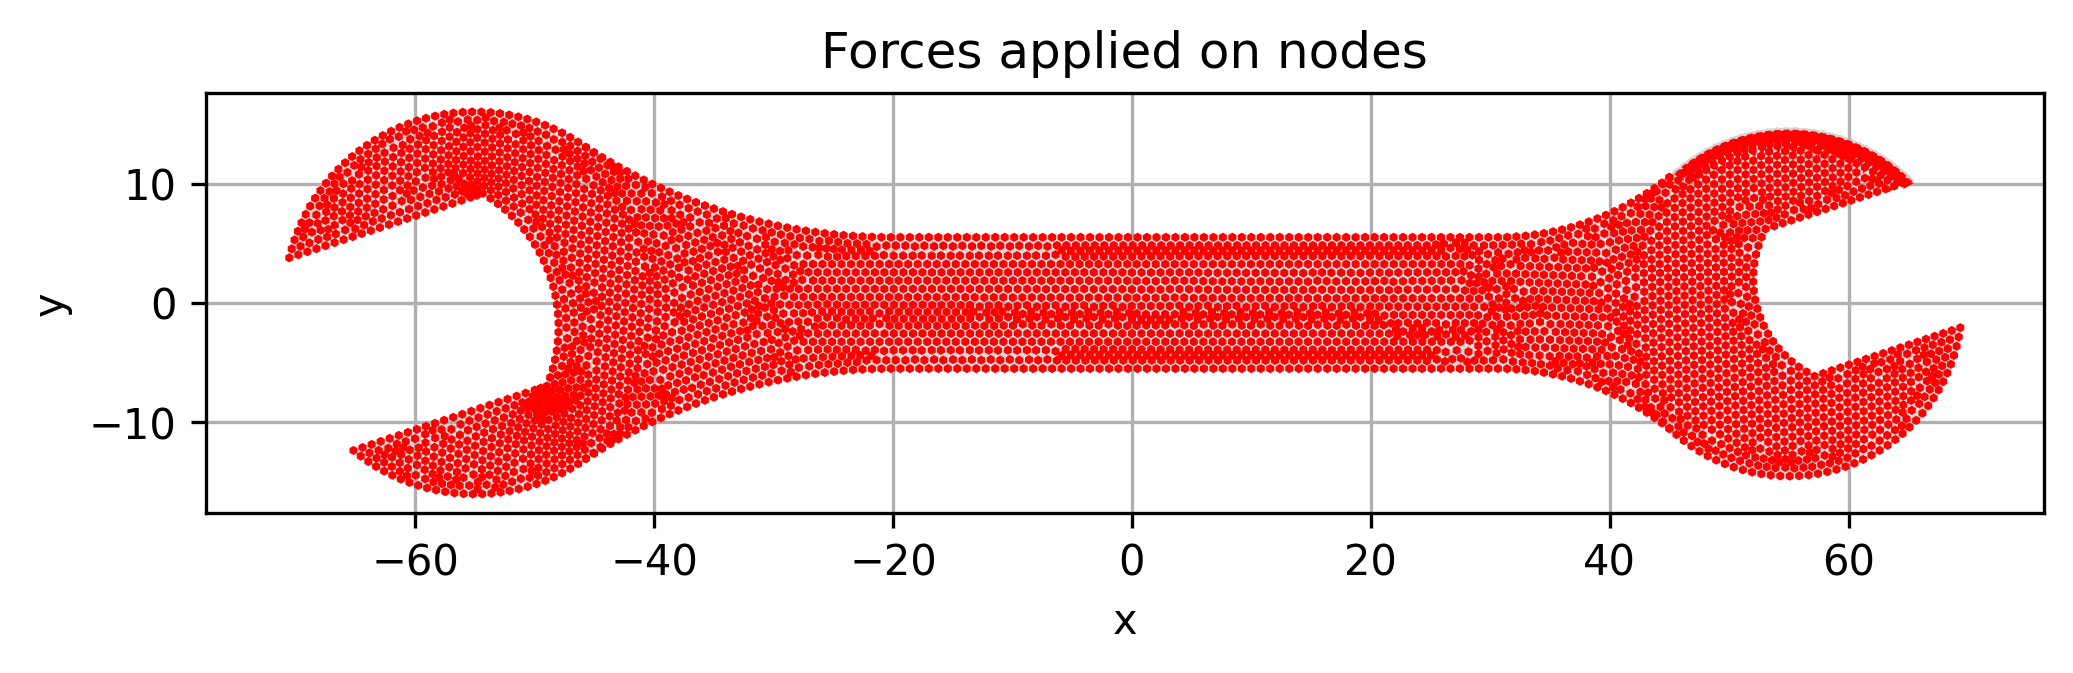
\includegraphics[width=0.8\textwidth]{GRAFICOS/Case c_fuerzas.png}
  \caption{Caption}
  \label{fig:strain}
\end{figure}

\begin{figure}[H]
  \centering
  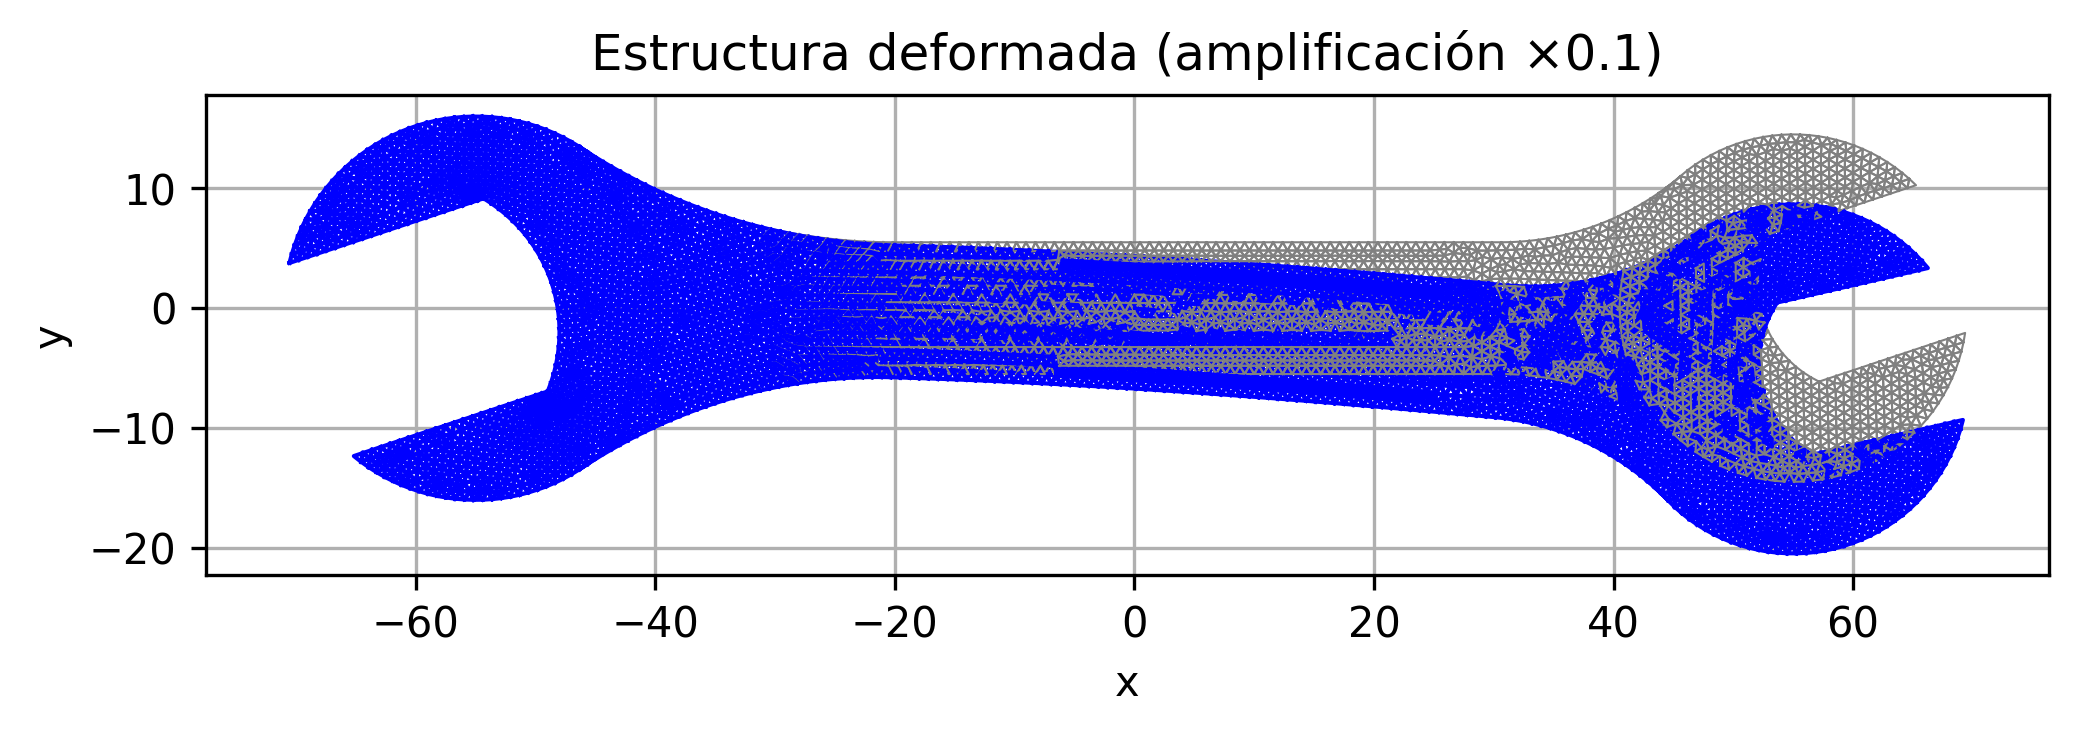
\includegraphics[width=0.8\textwidth]{GRAFICOS/Case c_deformada.png}
  \caption{Caption}
  \label{fig:stress}
\end{figure}

\begin{figure}[H]
  \centering
  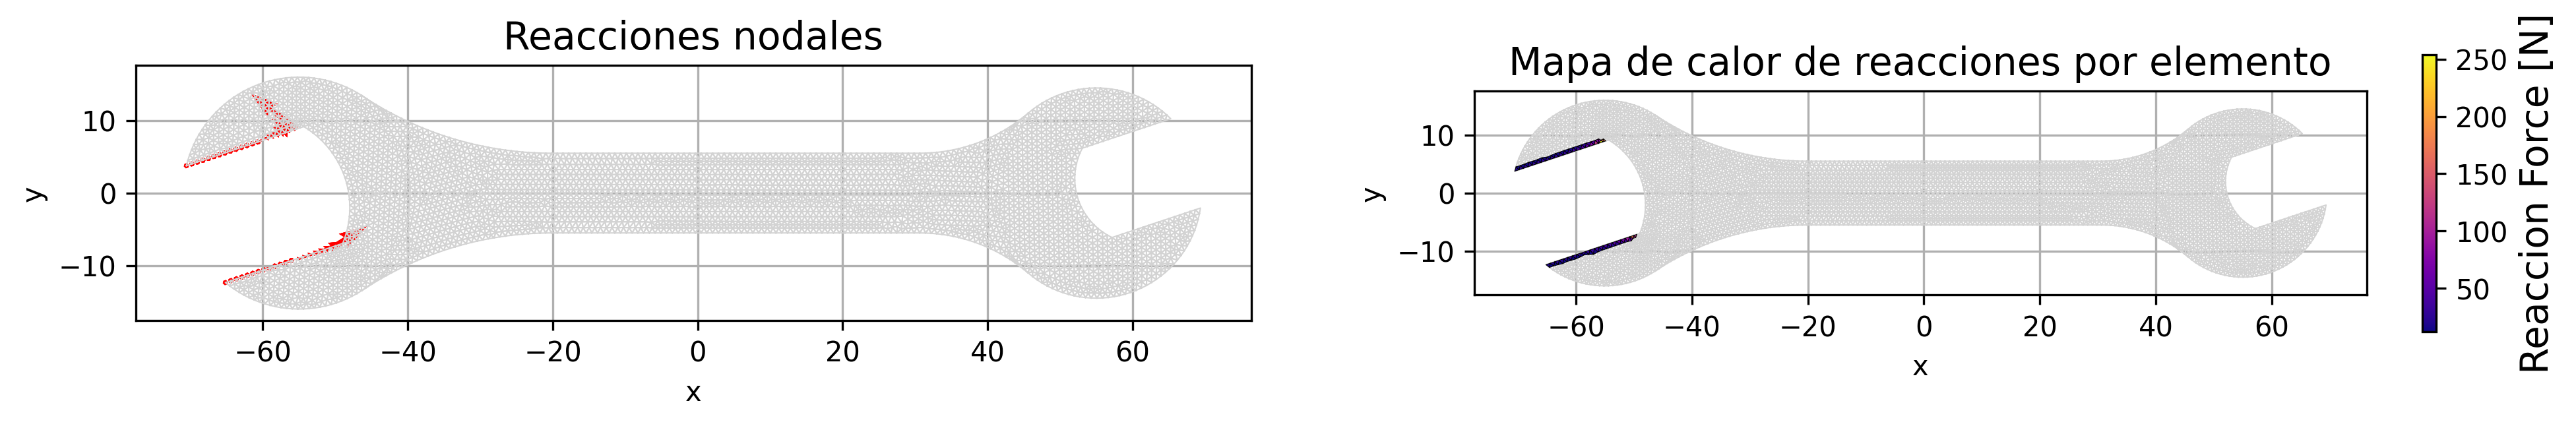
\includegraphics[width=1\textwidth]{GRAFICOS/Case c_deformada_reacciones.png}
  \caption{Caption}
  \label{fig:principal}
\end{figure}

\begin{figure}[H]
  \centering
  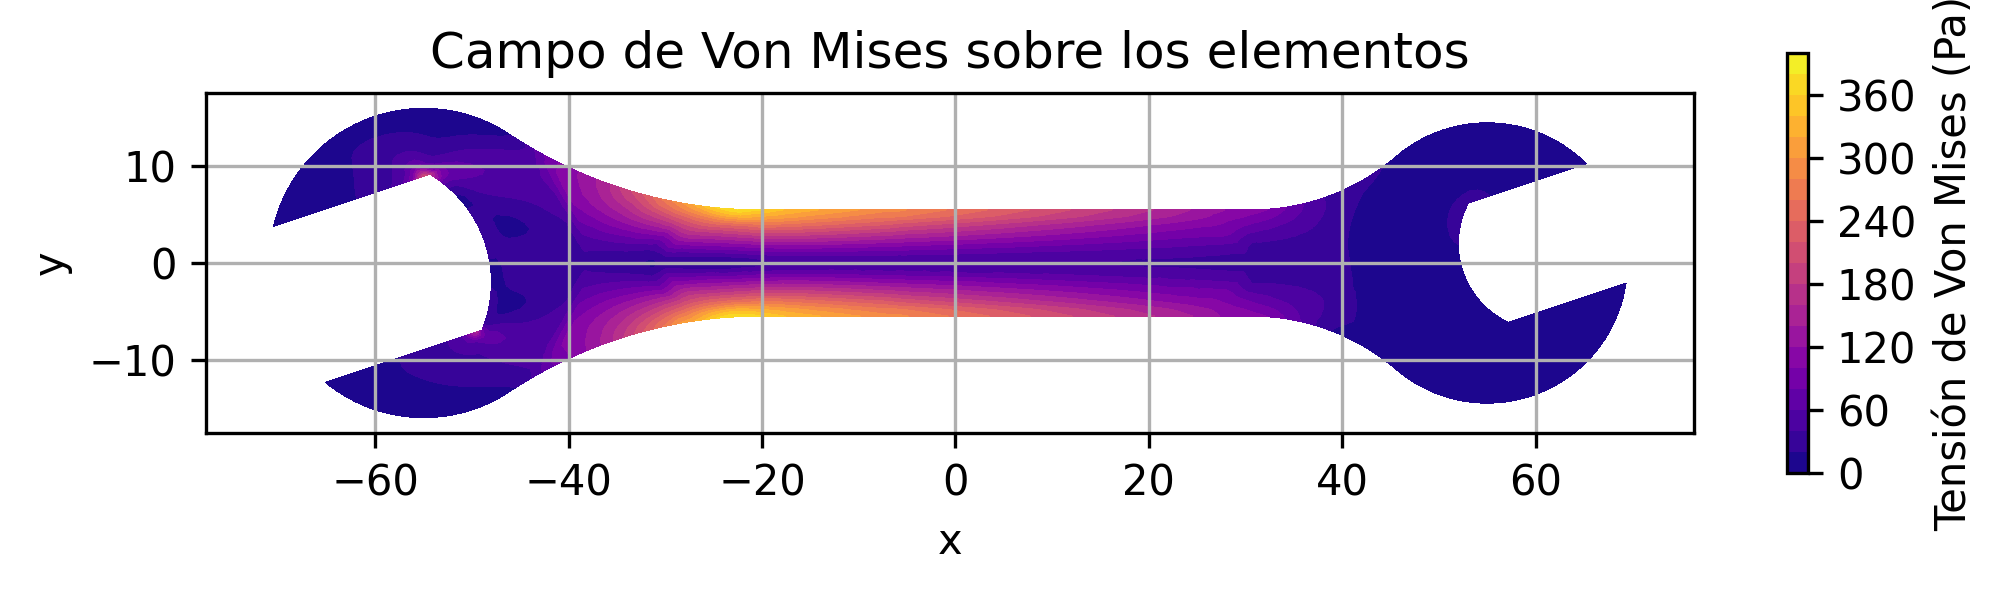
\includegraphics[width=0.8\textwidth]{GRAFICOS/Case c_von_mises.png}
  \caption{Caption}
  \label{fig:principal}
\end{figure}

\begin{figure}[H]
  \centering
  \begin{subfigure}[t]{0.49\textwidth}
    \centering
    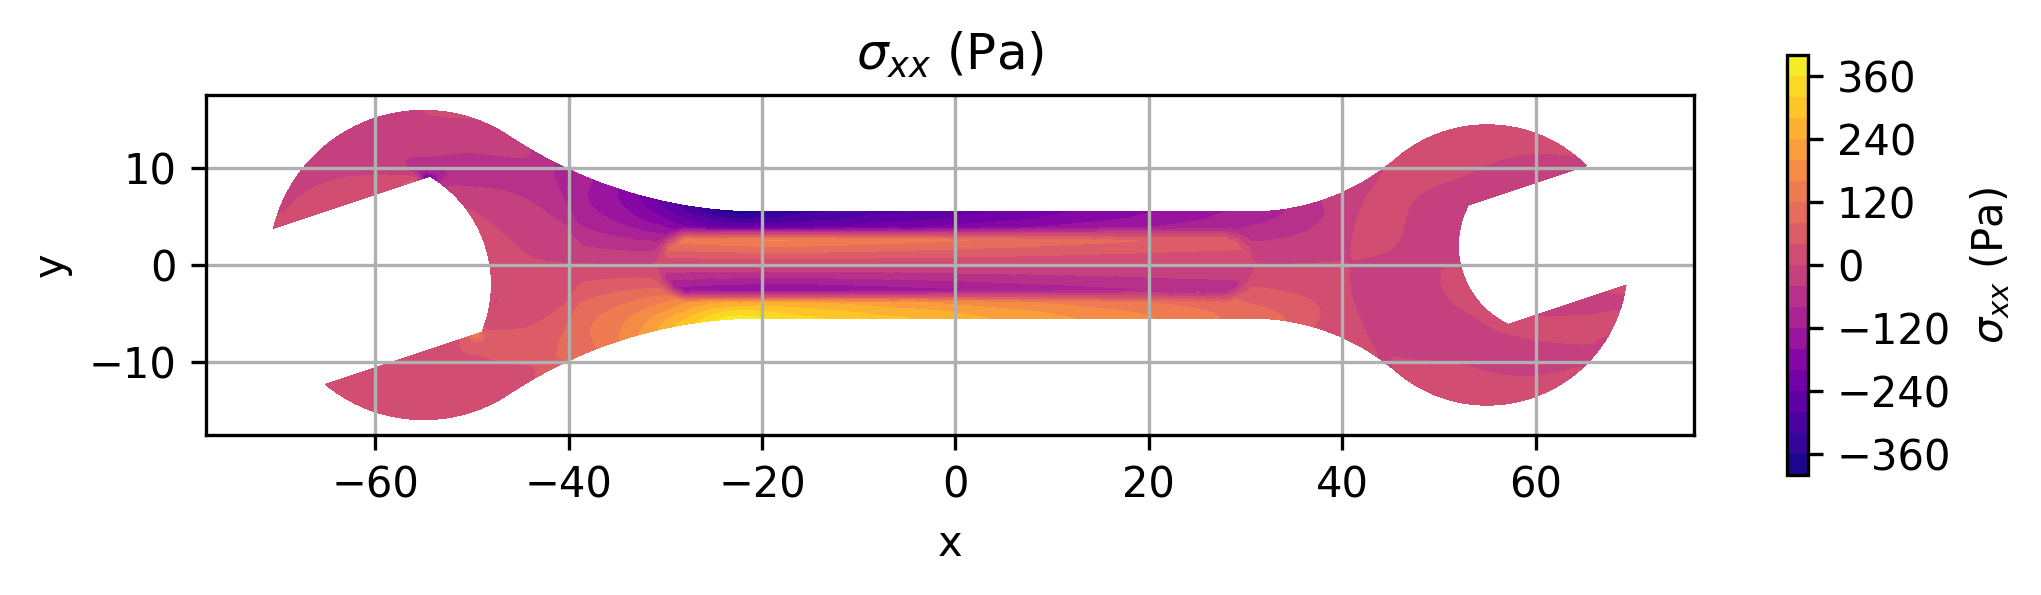
\includegraphics[width=\textwidth]{GRAFICOS/Case c - sigma_xx.png}
    \caption{Caption}
    \label{fig:deformada_reacciones}
  \end{subfigure}
  \hfill
  \begin{subfigure}[t]{0.49\textwidth}
    \centering
    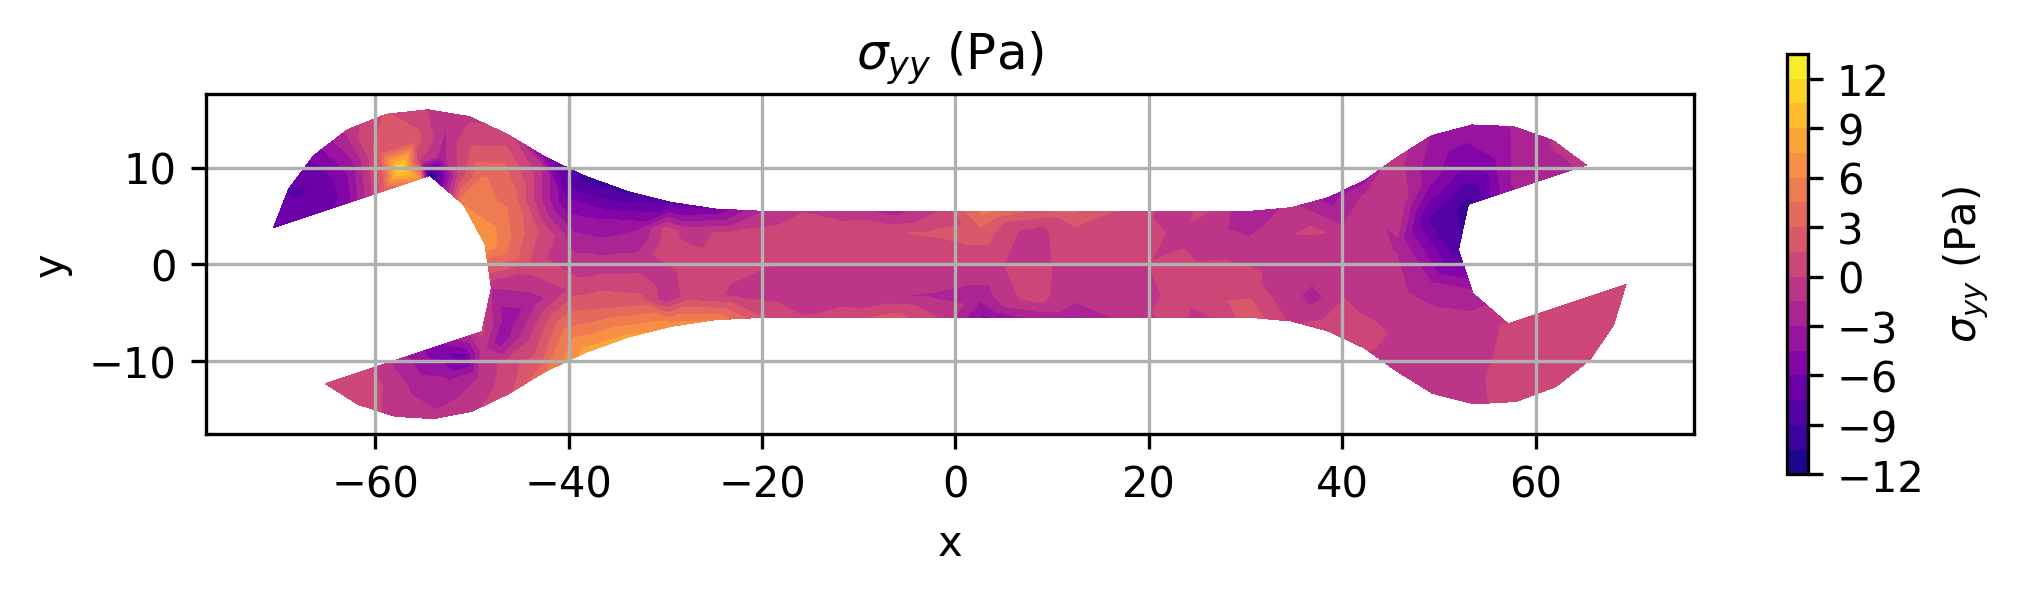
\includegraphics[width=\textwidth]{GRAFICOS/Case c - sigma_yy.png}
    \caption{Caption}
    \label{fig:von_mises}
  \end{subfigure}
  \caption{Caption}
  \label{fig:analisis_estructural}
\end{figure}

\begin{figure}[H]
  \centering
  \begin{subfigure}[t]{0.49\textwidth}
    \centering
    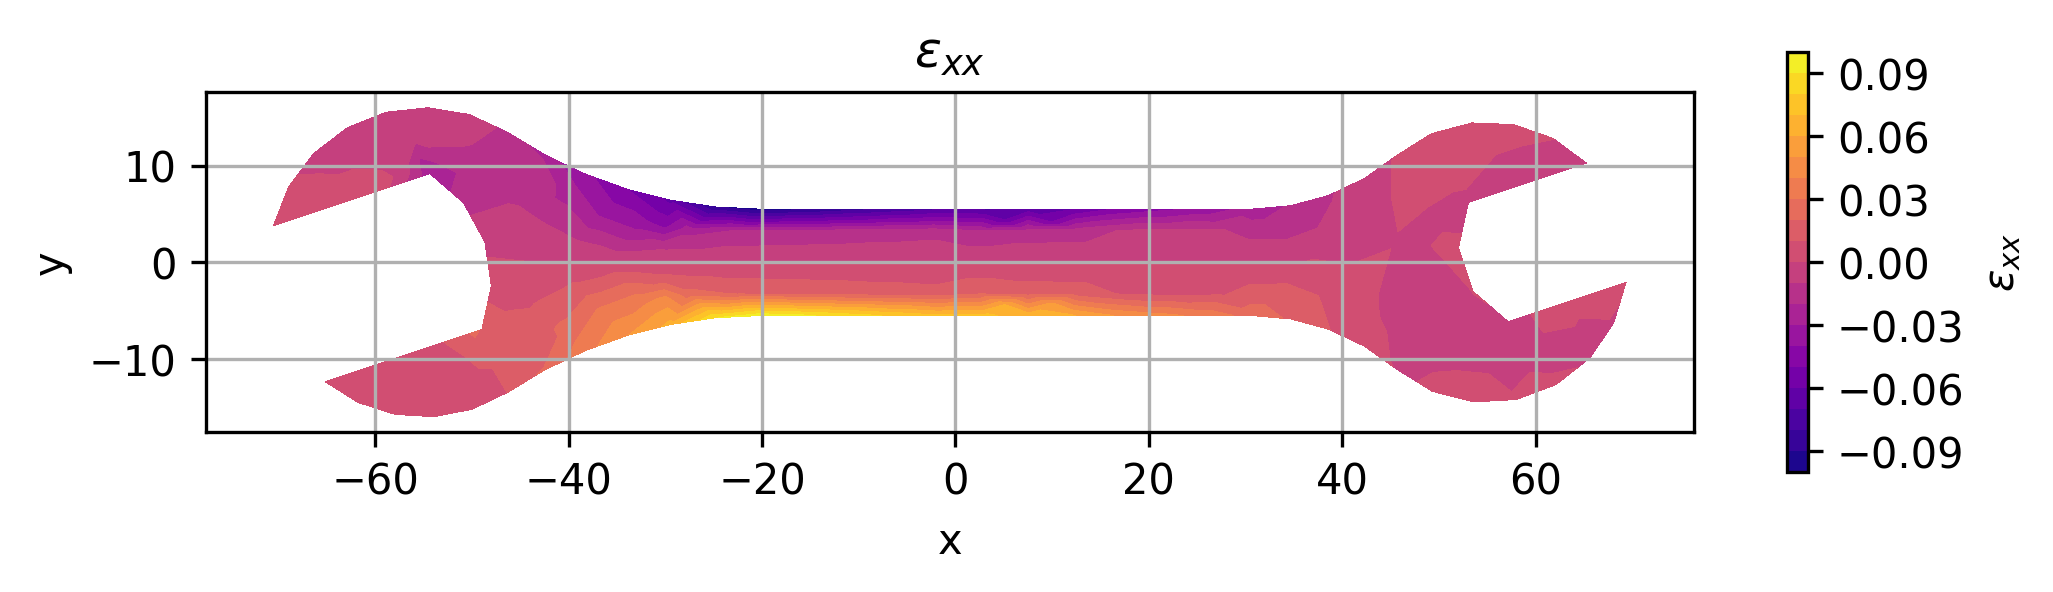
\includegraphics[width=\textwidth]{GRAFICOS/Case c - epsilon_xx.png}
    \caption{Caption}
    \label{fig:deformada_reacciones}
  \end{subfigure}
  \hfill
  \begin{subfigure}[t]{0.49\textwidth}
    \centering
    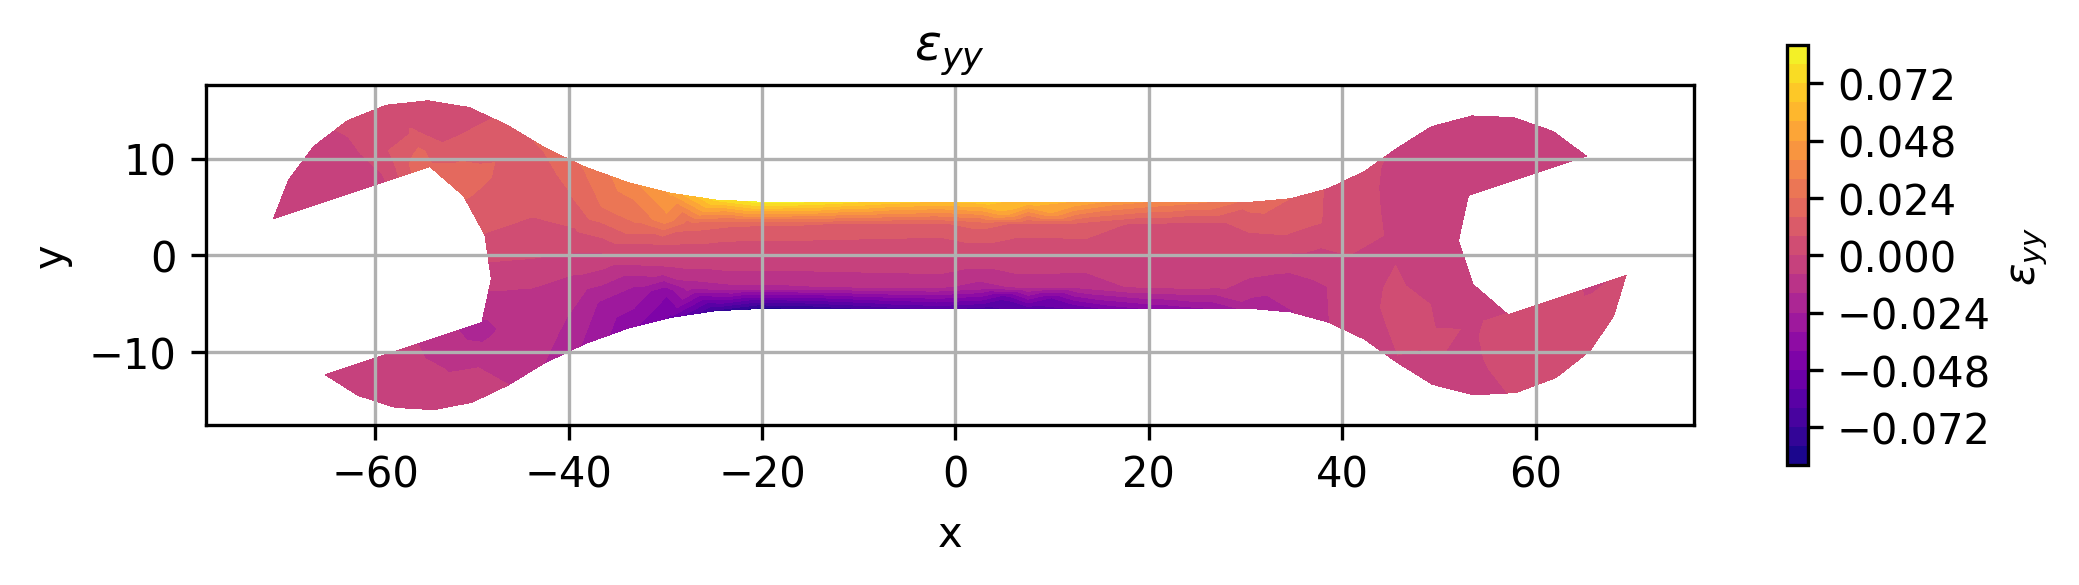
\includegraphics[width=\textwidth]{GRAFICOS/Case c - epsilon_yy.png}
    \caption{Caption}
    \label{fig:von_mises}
  \end{subfigure}
  \caption{Caption}
  \label{fig:analisis_estructural}
\end{figure}


\begin{figure}[H]
  \centering
  \begin{subfigure}[t]{0.49\textwidth}
    \centering
    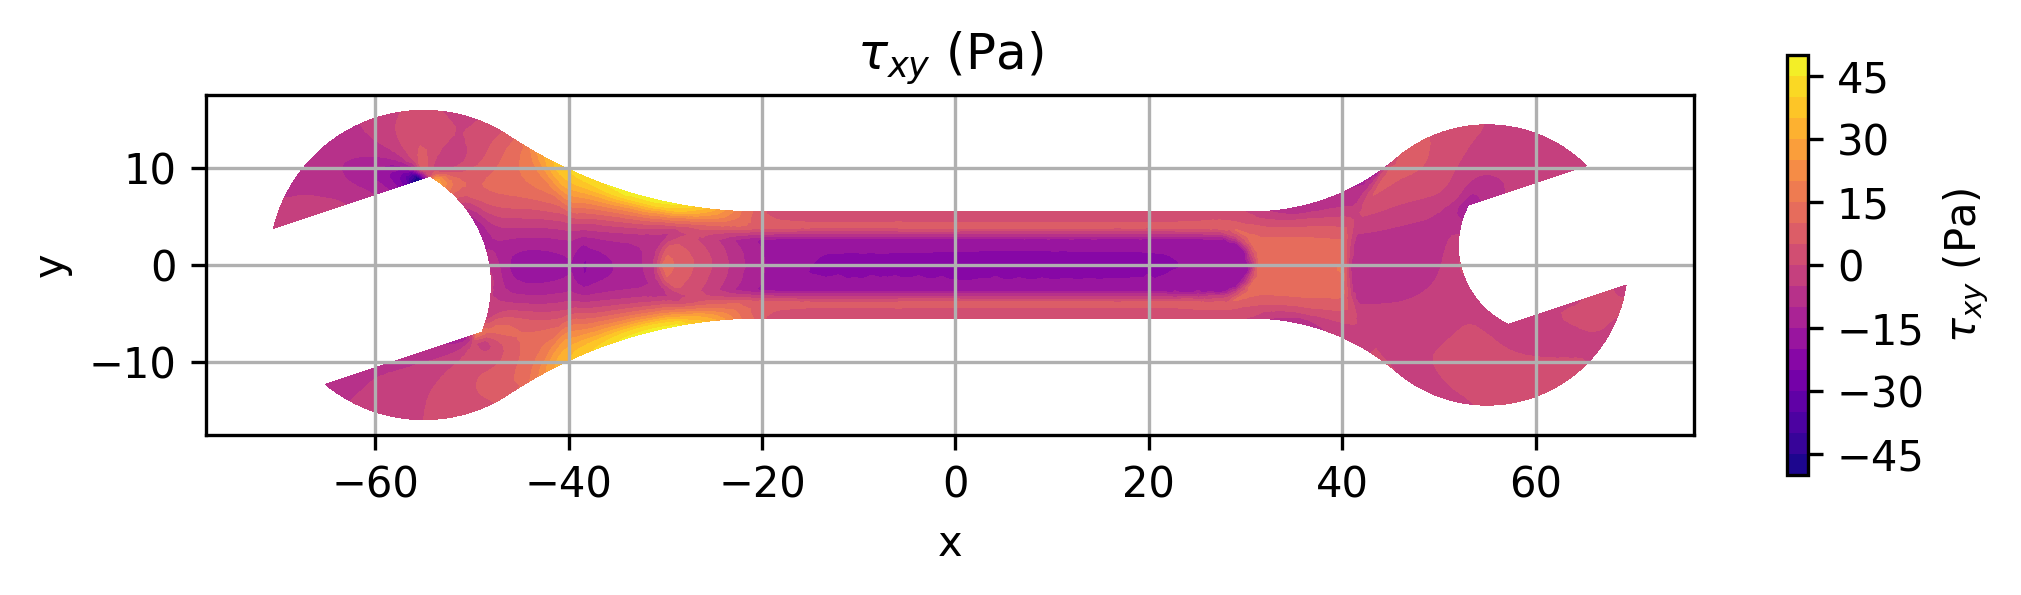
\includegraphics[width=\textwidth]{GRAFICOS/Case c - tau_xy.png}
    \caption{Caption}
    \label{fig:deformada_reacciones}
  \end{subfigure}
  \hfill
  \begin{subfigure}[t]{0.49\textwidth}
    \centering
    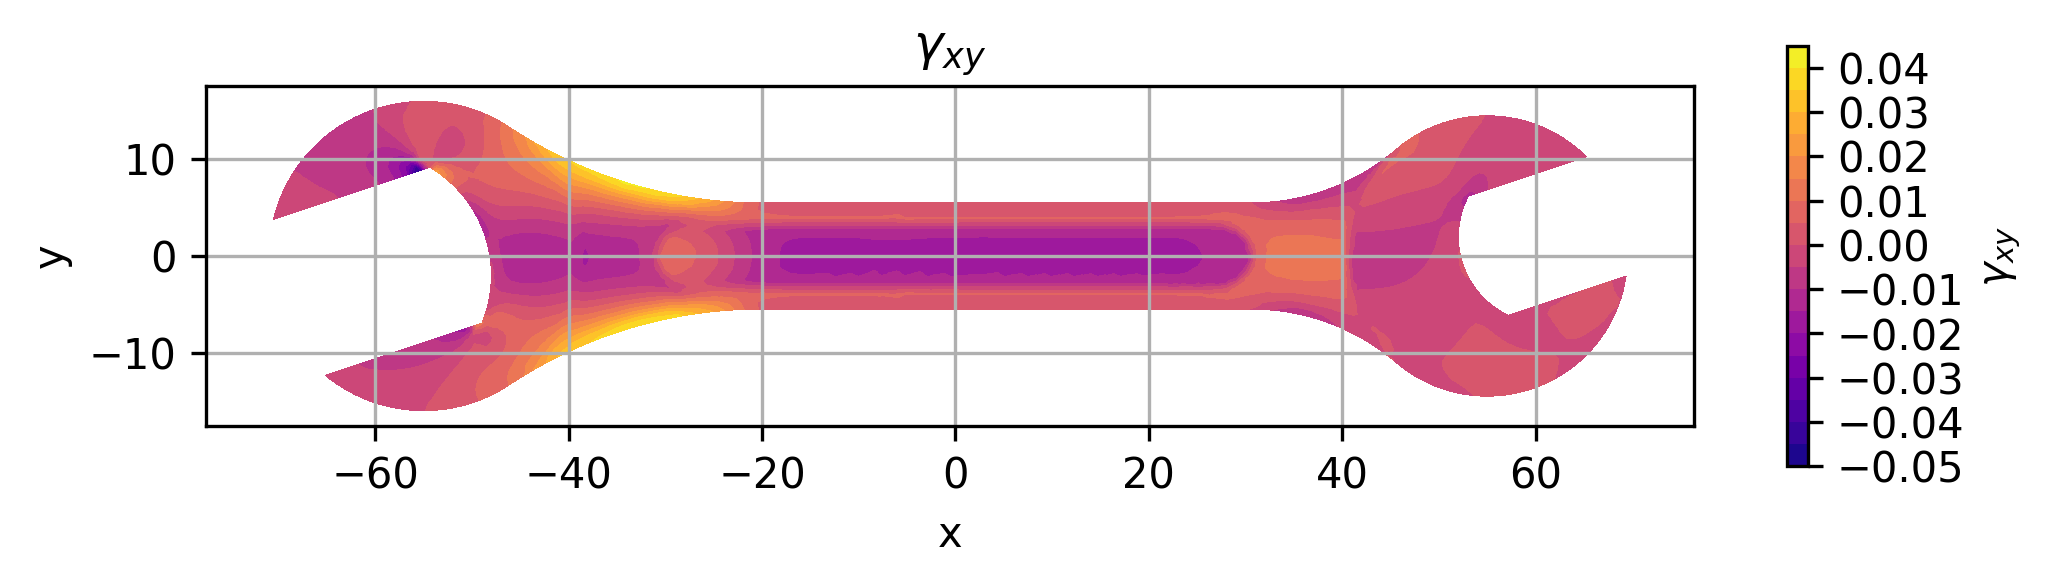
\includegraphics[width=\textwidth]{GRAFICOS/Case c - gamma_xy.png}
    \caption{Caption}
    \label{fig:von_mises}
  \end{subfigure}
  \caption{Caption}
  \label{fig:analisis_estructural}
\end{figure}

\begin{figure}[H]
  \centering
  \begin{subfigure}[t]{0.49\textwidth}
    \centering
    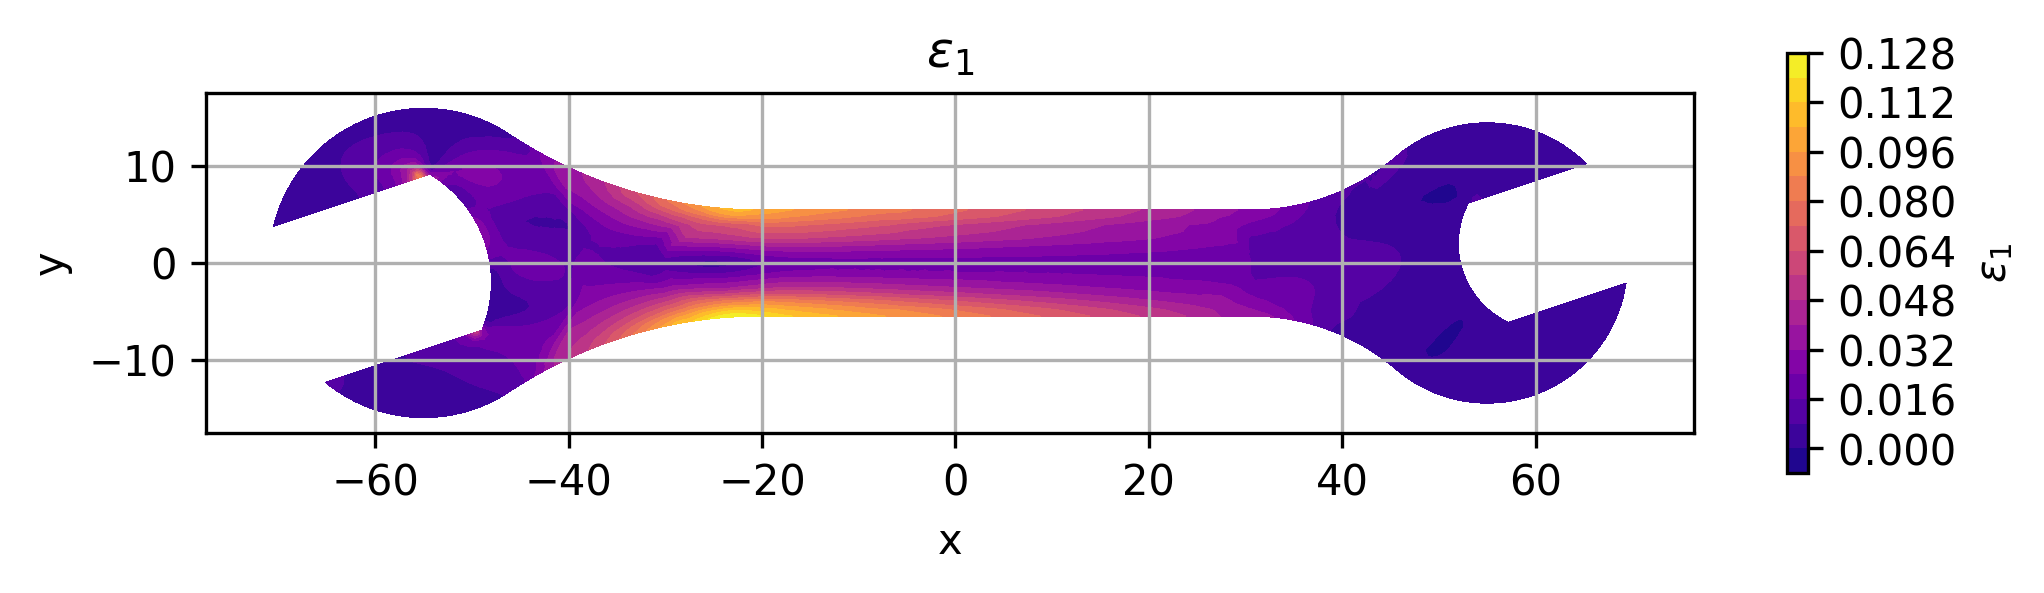
\includegraphics[width=\textwidth]{GRAFICOS/Case c - epsilon_1.png}
    \caption{Caption}
    \label{fig:deformada_reacciones}
  \end{subfigure}
  \hfill
  \begin{subfigure}[t]{0.49\textwidth}
    \centering
    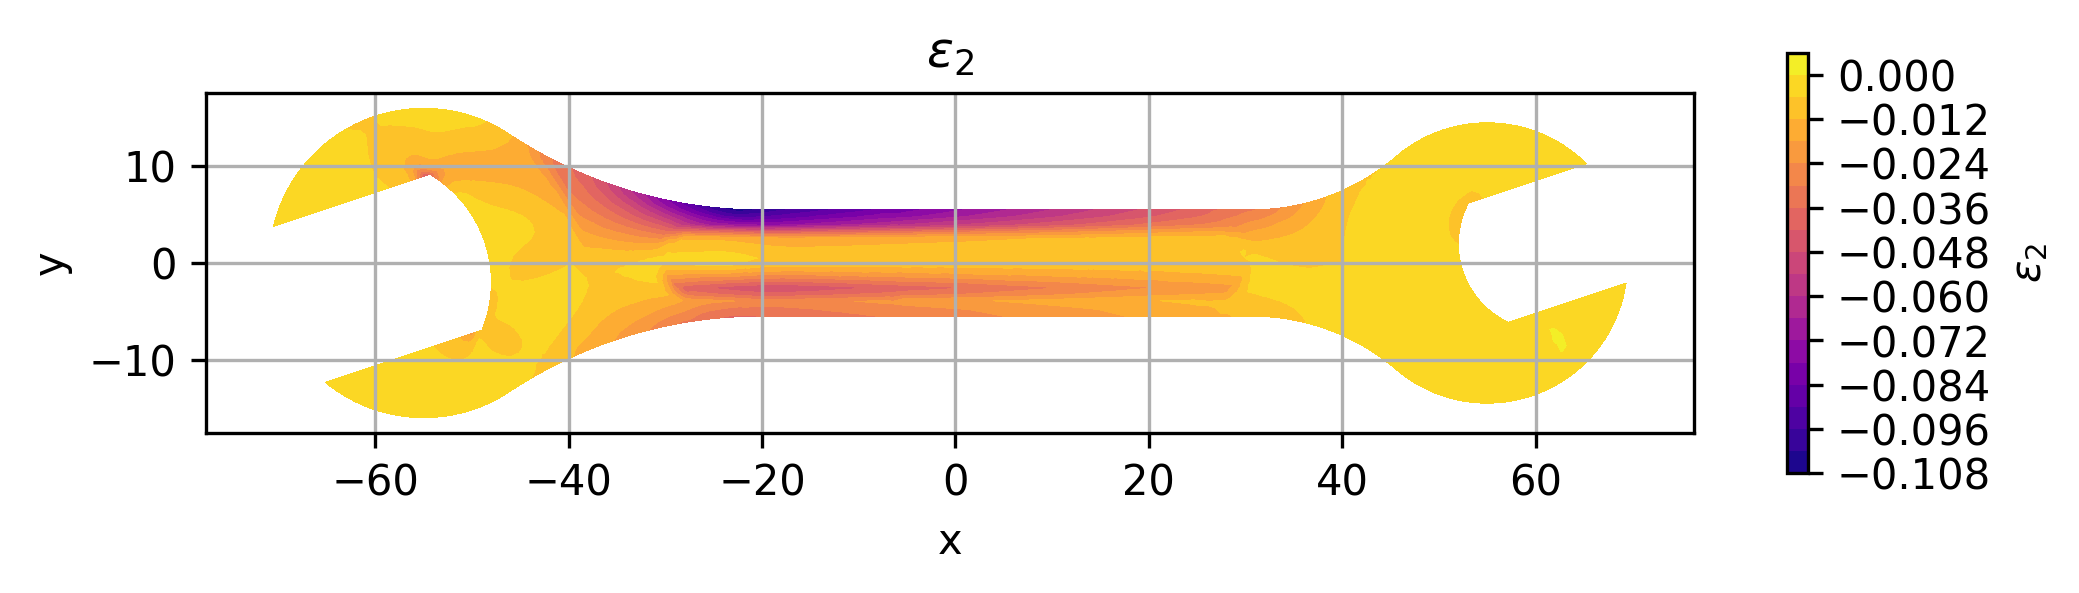
\includegraphics[width=\textwidth]{GRAFICOS/Case c - epsilon_2.png}
    \caption{Caption}
    \label{fig:von_mises}
  \end{subfigure}
  \caption{Caption}
  \label{fig:analisis_estructural}
\end{figure}

\begin{figure}[H]
  \centering
  \begin{subfigure}[t]{0.49\textwidth}
    \centering
    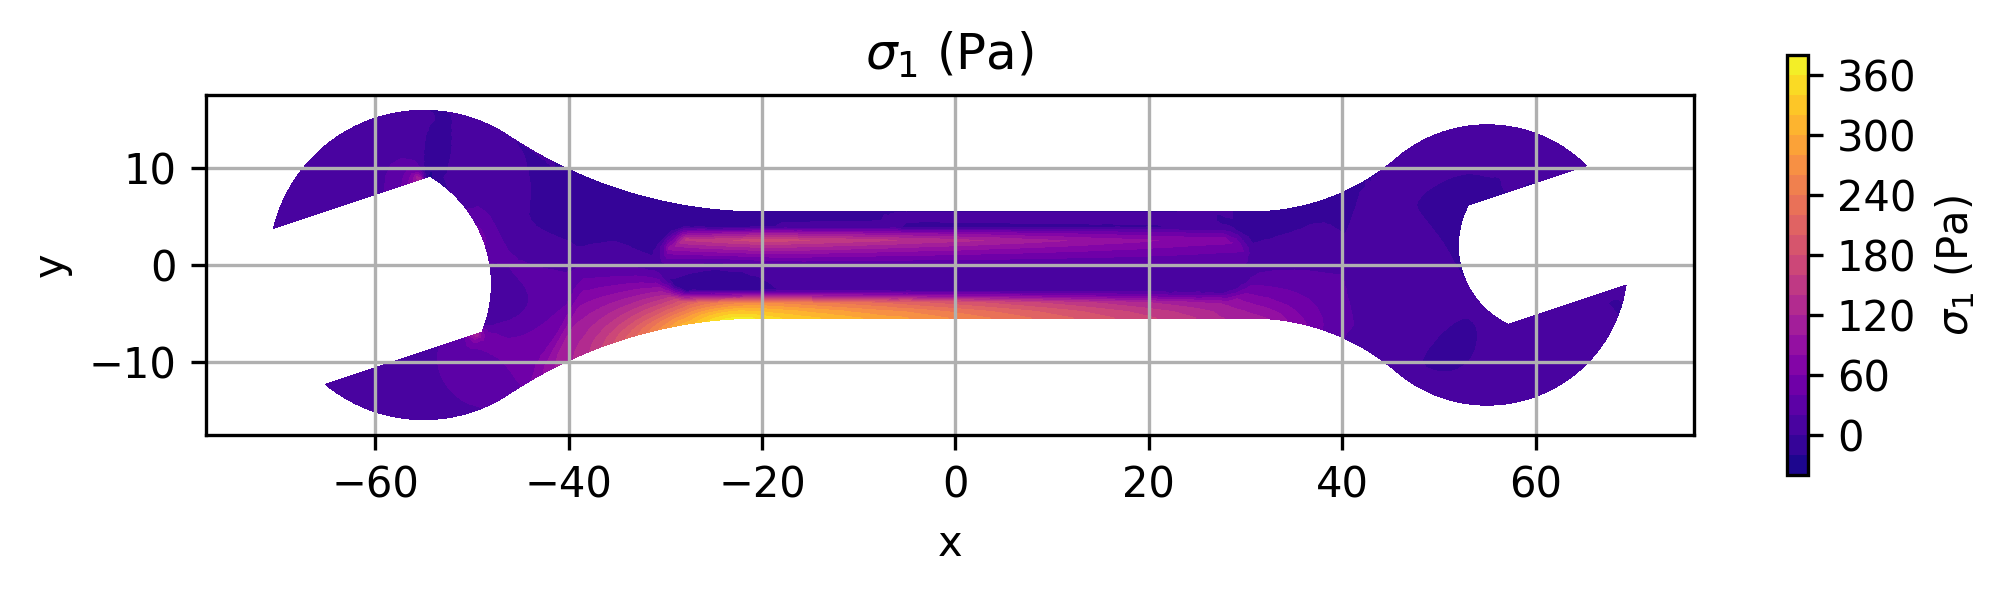
\includegraphics[width=\textwidth]{GRAFICOS/Case c - sigma_1.png}
    \caption{Caption}
    \label{fig:deformada_reacciones}
  \end{subfigure}
  \hfill
  \begin{subfigure}[t]{0.49\textwidth}
    \centering
    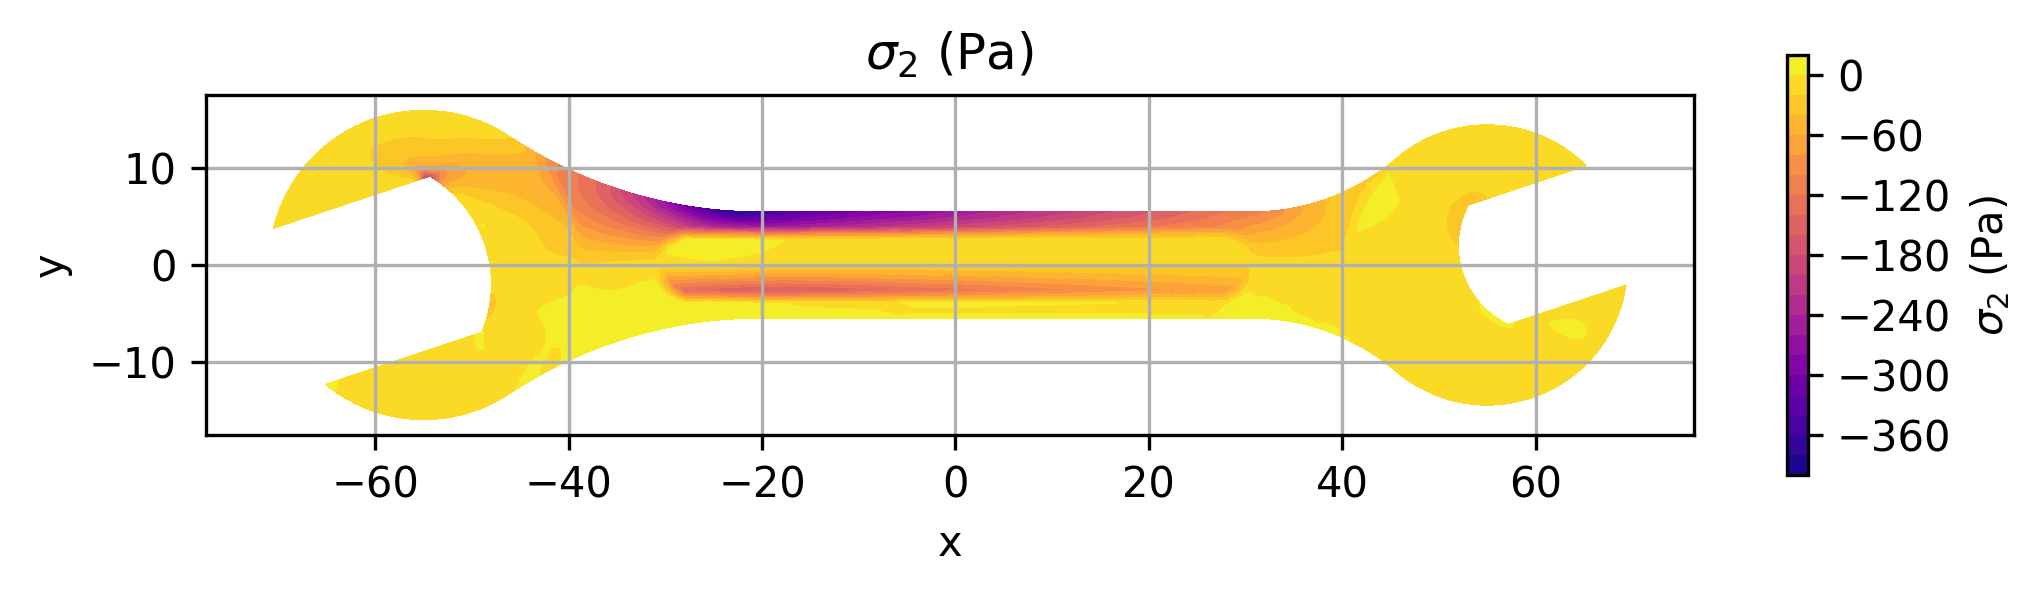
\includegraphics[width=\textwidth]{GRAFICOS/Case c - sigma_2.png}
    \caption{Caption}
    \label{fig:von_mises}
  \end{subfigure}
  \caption{Caption}
  \label{fig:analisis_estructural}
\end{figure}

\section{D case, only self weight}

\begin{figure}[H]
  \centering
  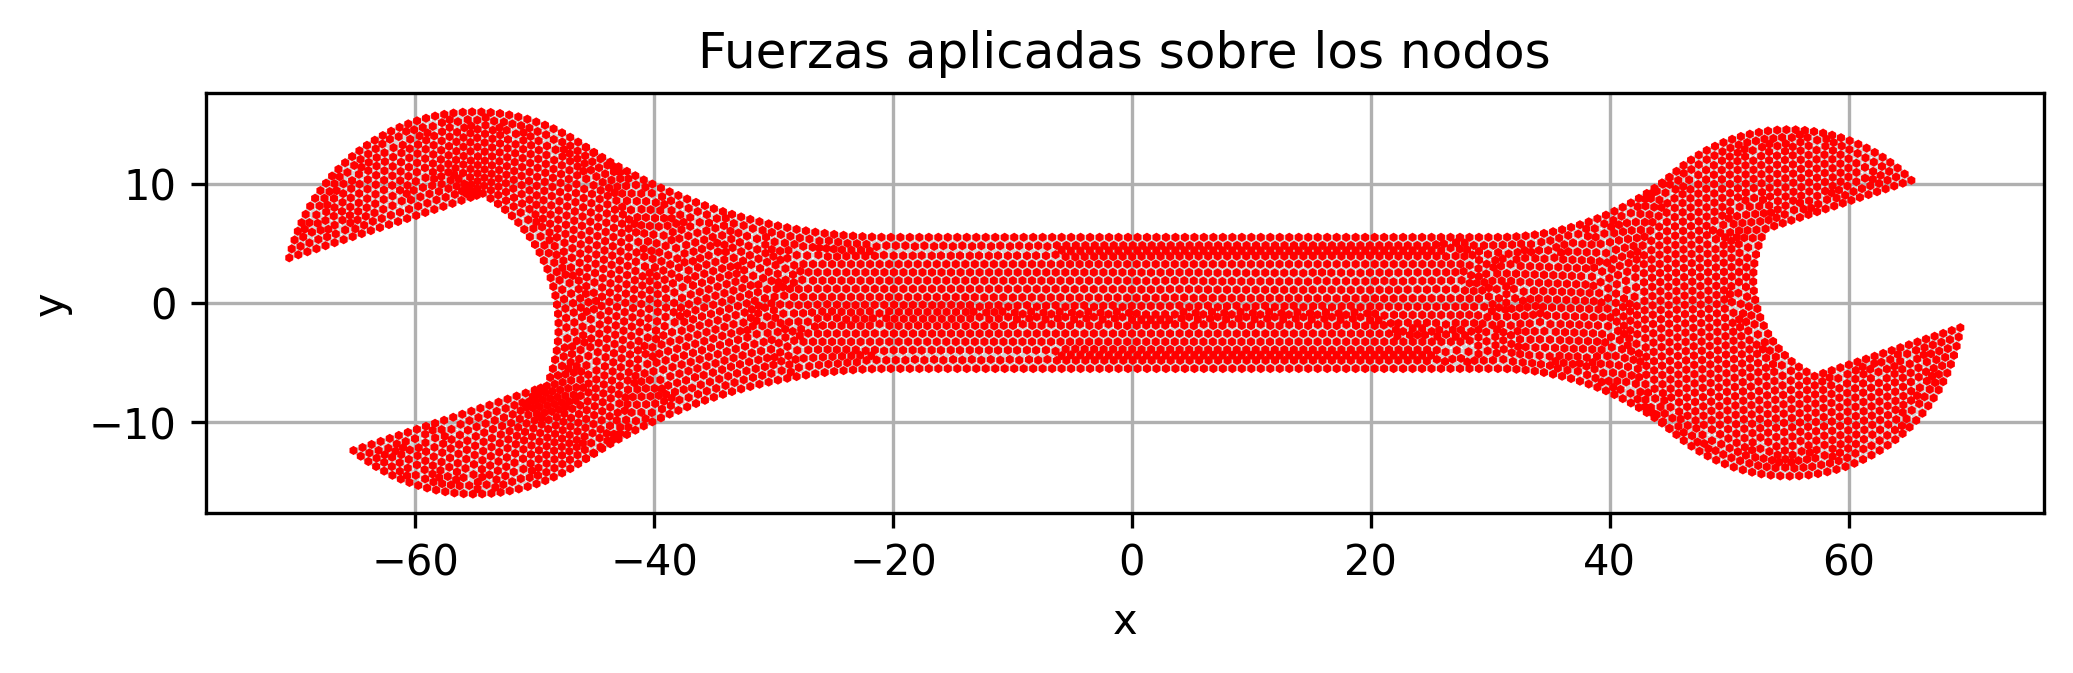
\includegraphics[width=0.8\textwidth]{GRAFICOS/Case d_fuerzas.png}
  \caption{Caption}
  \label{fig:strain}
\end{figure}

\begin{figure}[H]
  \centering
  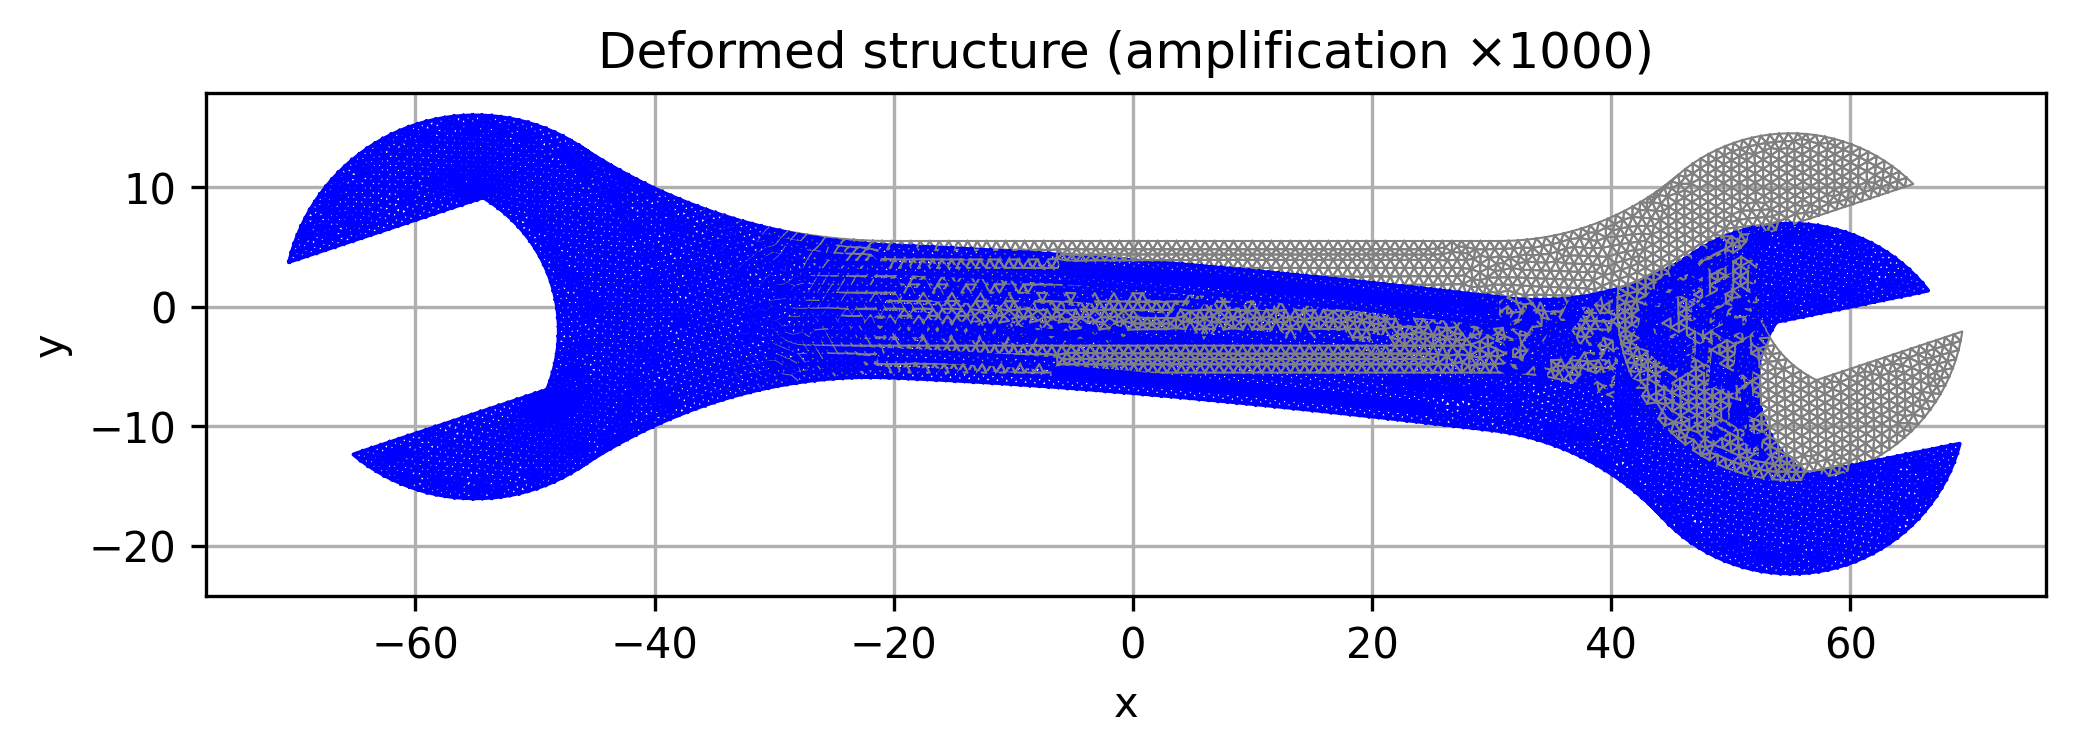
\includegraphics[width=0.8\textwidth]{GRAFICOS/Case d_deformada.png}
  \caption{Caption}
  \label{fig:stress}
\end{figure}

\begin{figure}[H]
  \centering
  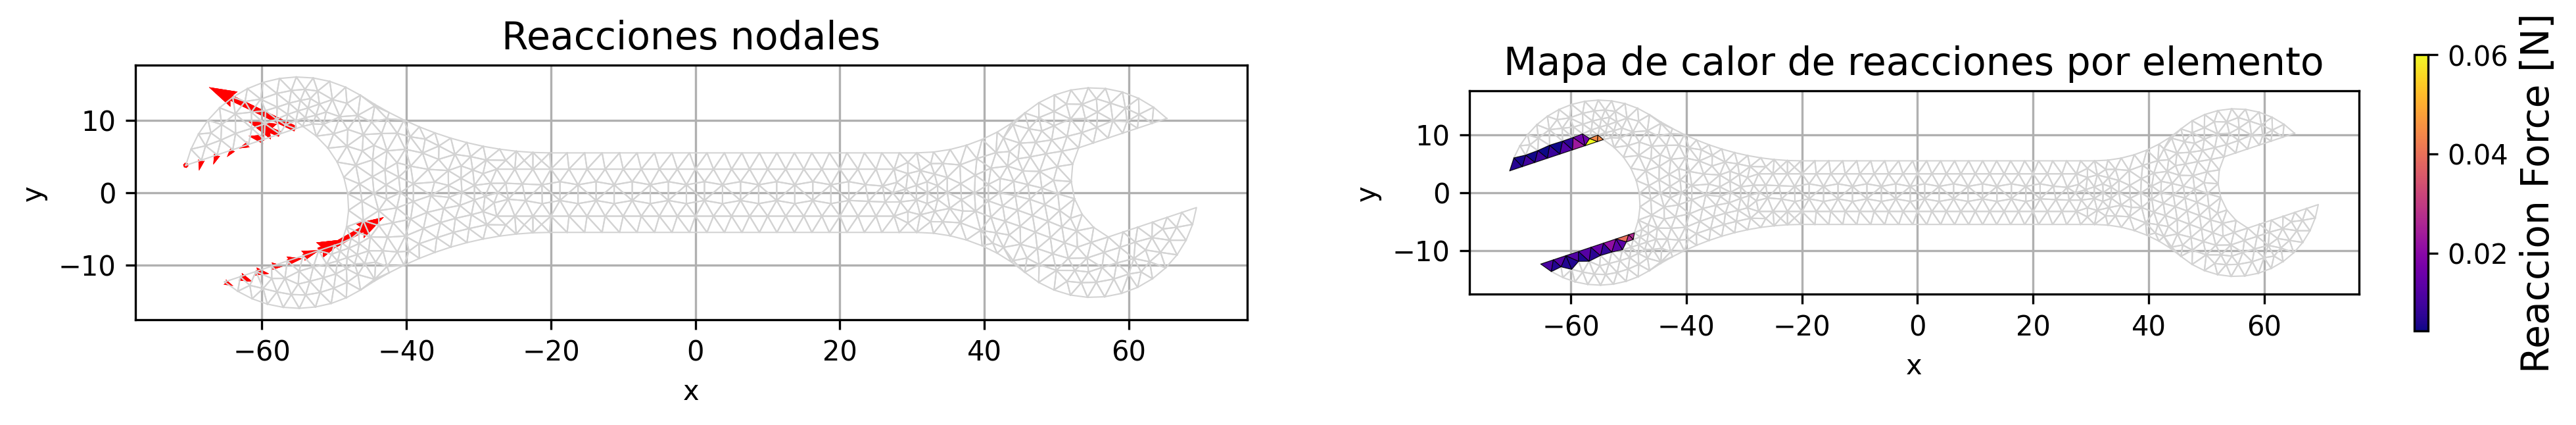
\includegraphics[width=1\textwidth]{GRAFICOS/Case d_deformada_reacciones.png}
  \caption{Caption}
  \label{fig:principal}
\end{figure}

\begin{figure}[H]
  \centering
  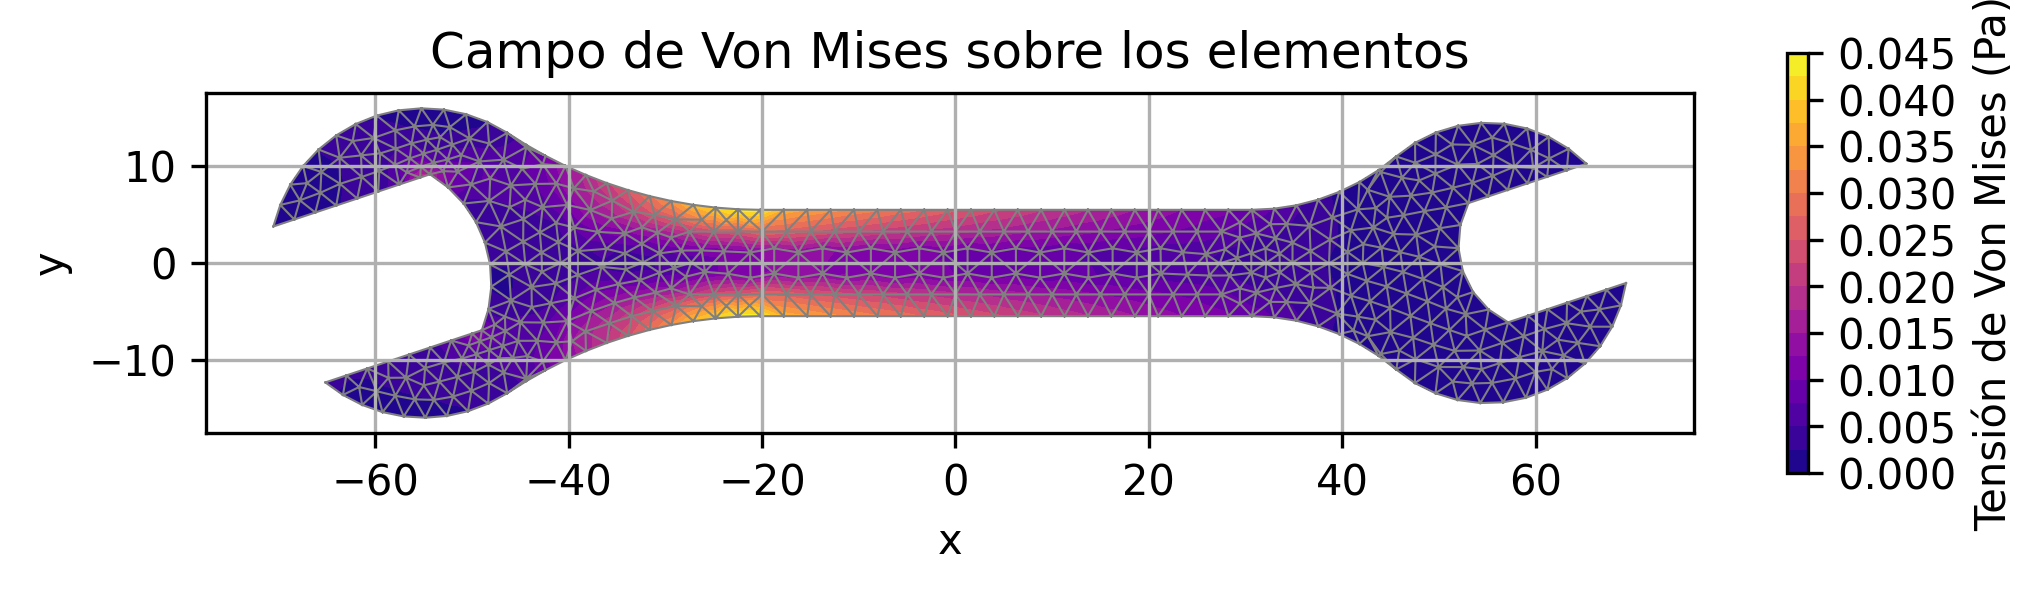
\includegraphics[width=0.8\textwidth]{GRAFICOS/Case d_von_mises.png}
  \caption{Caption}
  \label{fig:principal}
\end{figure}

\begin{figure}[H]
  \centering
  \begin{subfigure}[t]{0.49\textwidth}
    \centering
    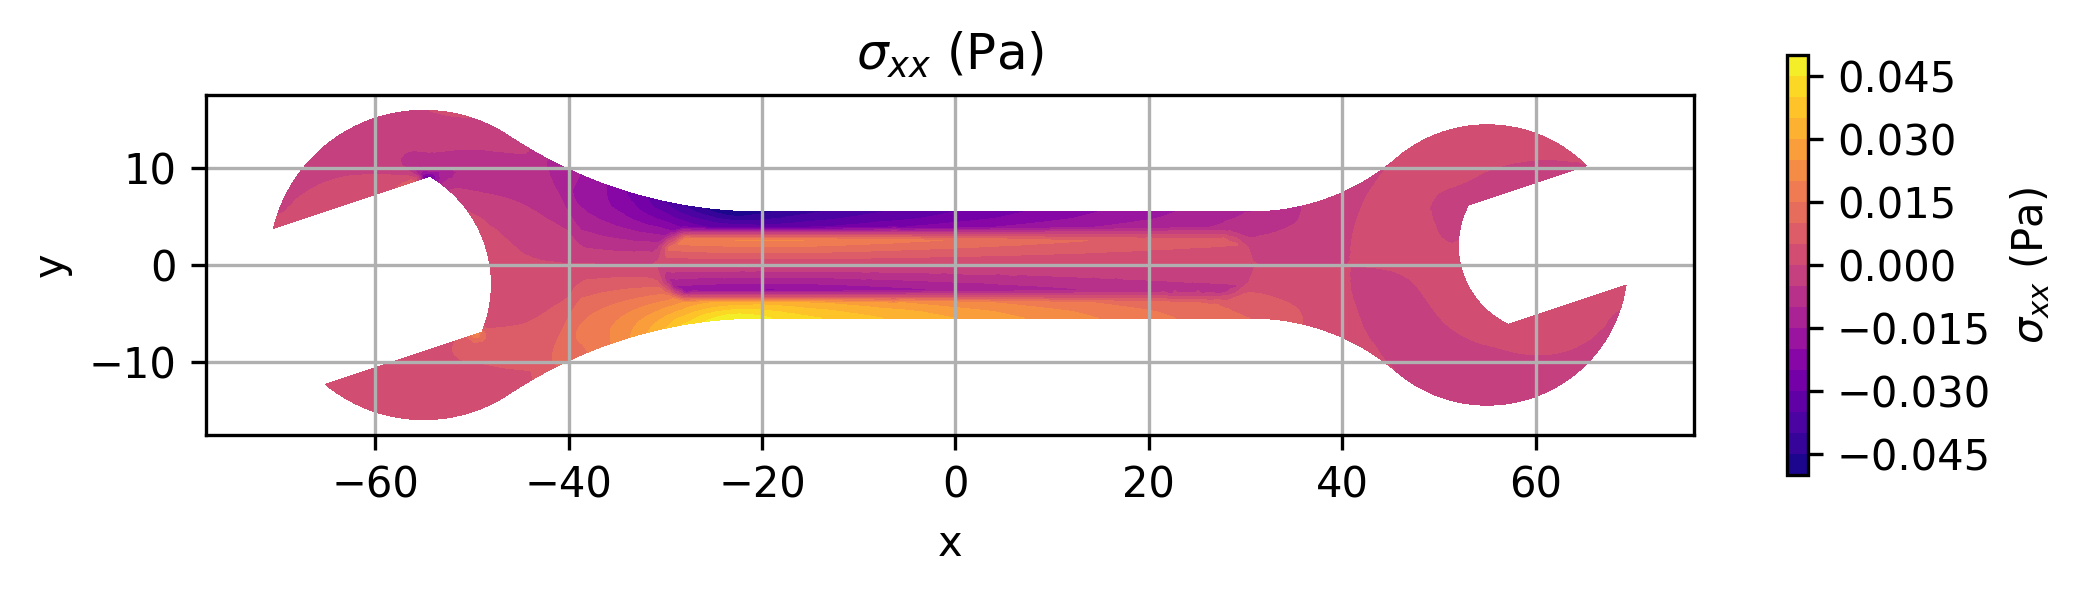
\includegraphics[width=\textwidth]{GRAFICOS/Case d - sigma_xx.png}
    \caption{Caption}
    \label{fig:deformada_reacciones}
  \end{subfigure}
  \hfill
  \begin{subfigure}[t]{0.49\textwidth}
    \centering
    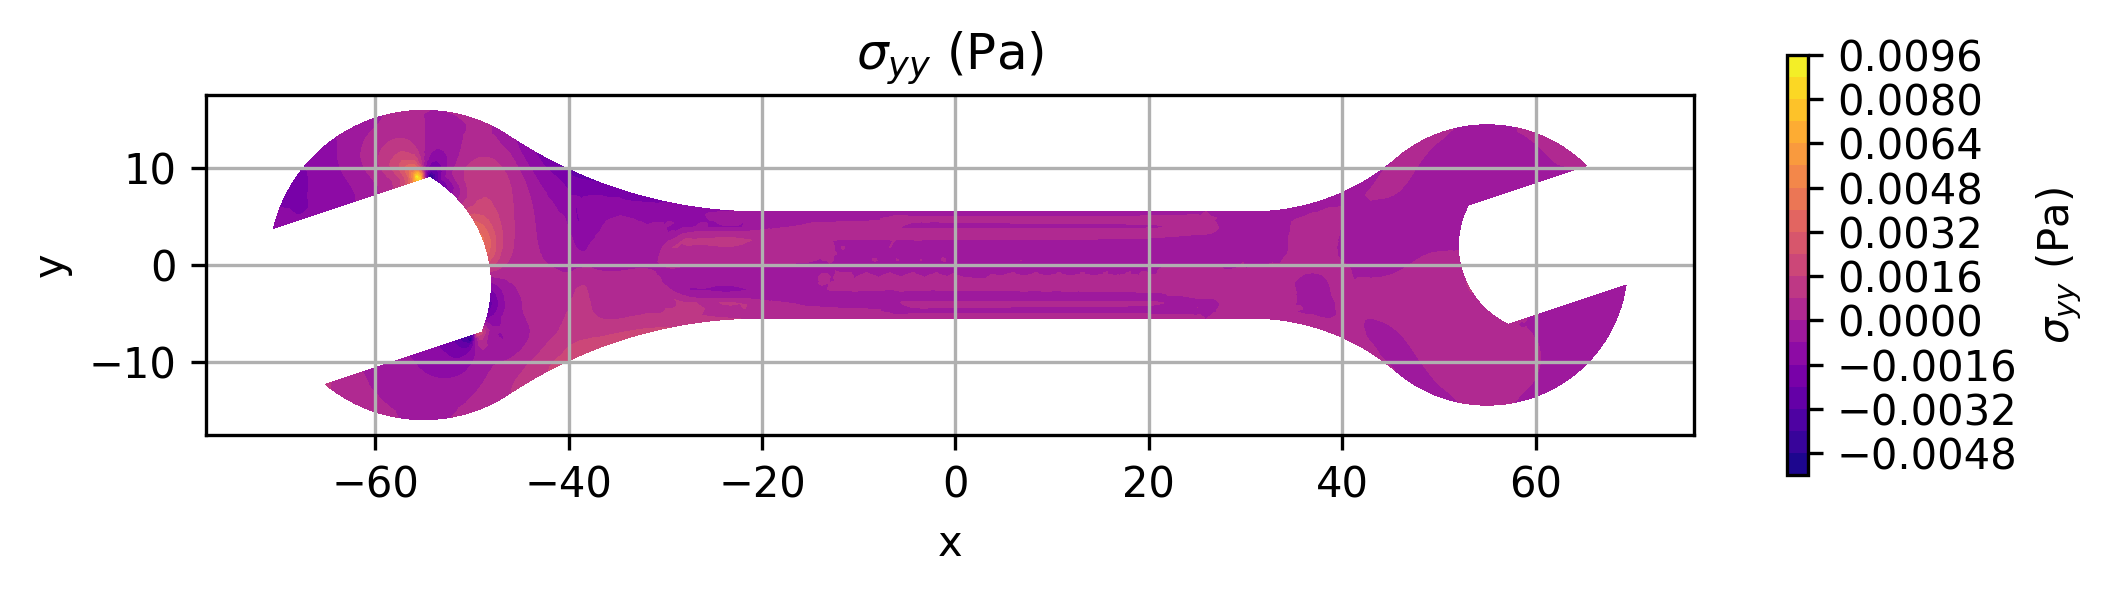
\includegraphics[width=\textwidth]{GRAFICOS/Case d - sigma_yy.png}
    \caption{Caption}
    \label{fig:von_mises}
  \end{subfigure}
  \caption{Caption}
  \label{fig:analisis_estructural}
\end{figure}

\begin{figure}[H]
  \centering
  \begin{subfigure}[t]{0.49\textwidth}
    \centering
    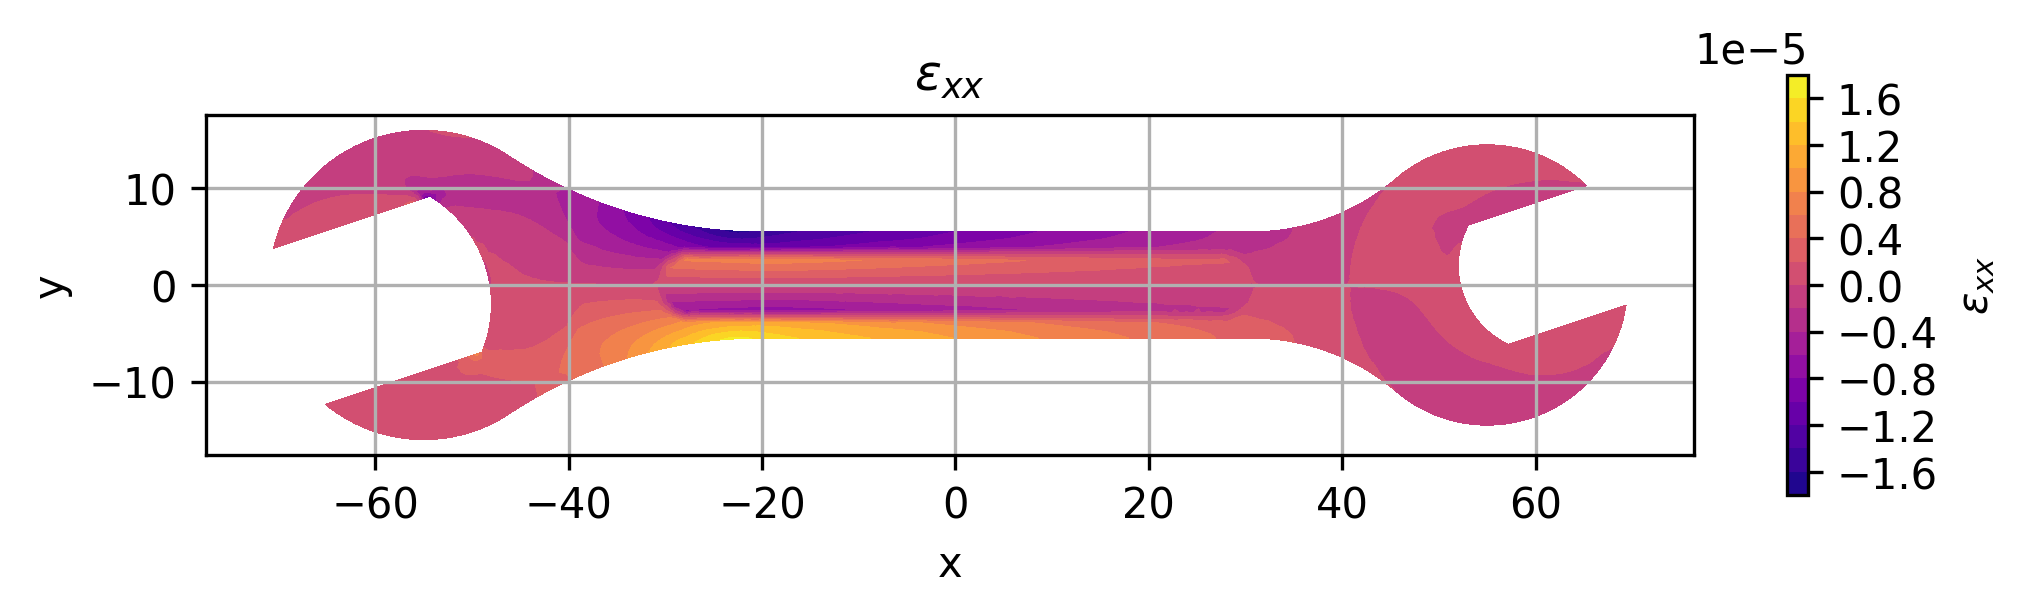
\includegraphics[width=\textwidth]{GRAFICOS/Case d - epsilon_xx.png}
    \caption{Caption}
    \label{fig:deformada_reacciones}
  \end{subfigure}
  \hfill
  \begin{subfigure}[t]{0.49\textwidth}
    \centering
    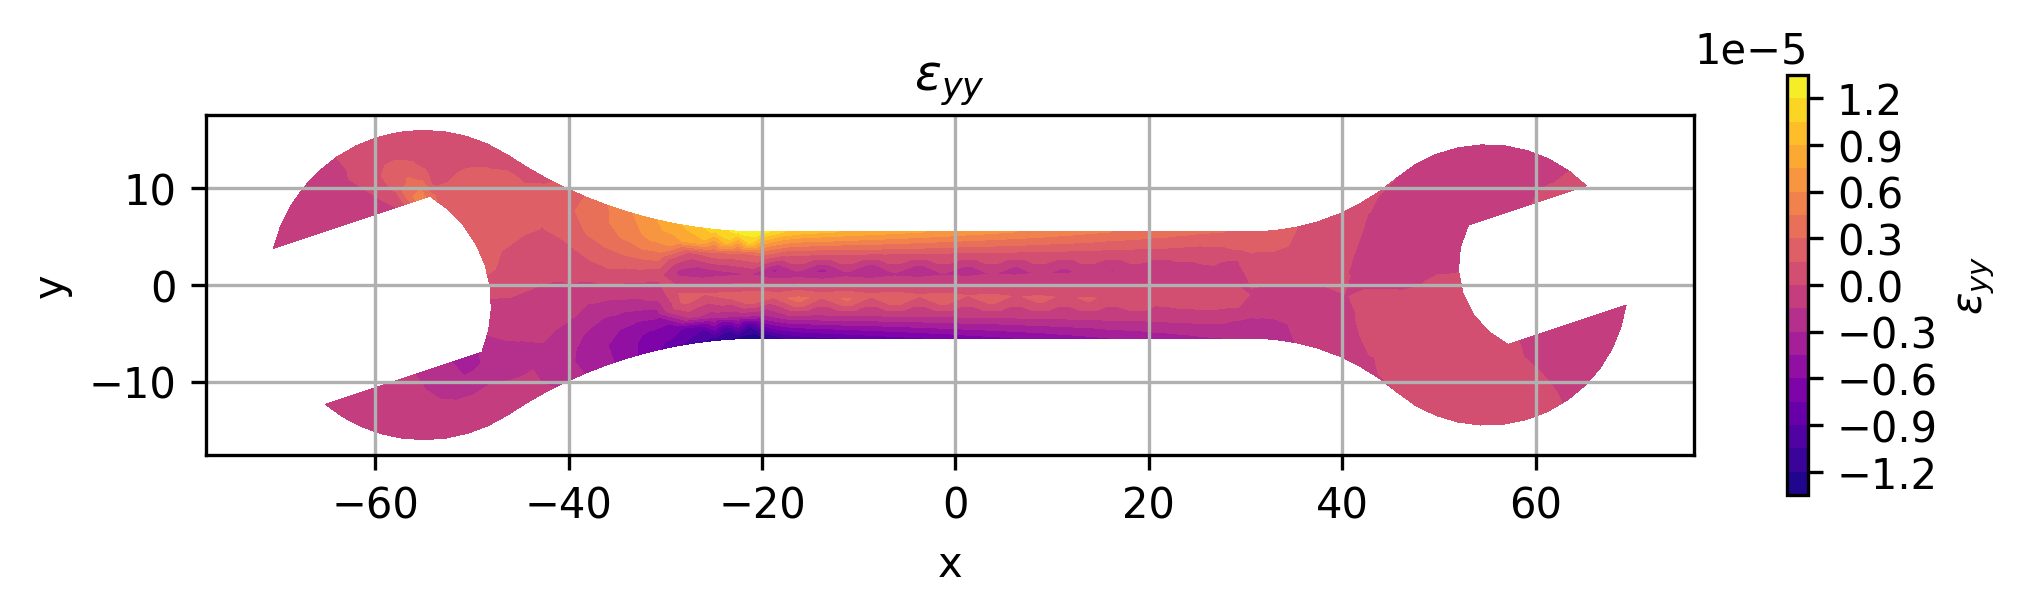
\includegraphics[width=\textwidth]{GRAFICOS/Case d - epsilon_yy.png}
    \caption{Caption}
    \label{fig:von_mises}
  \end{subfigure}
  \caption{Caption}
  \label{fig:analisis_estructural}
\end{figure}

\begin{figure}[H]
  \centering
  \begin{subfigure}[t]{0.49\textwidth}
    \centering
    \includegraphics[width=\textwidth]{GRAFICOS/Case d - tau_xy.png}
    \caption{Caption}
    \label{fig:deformada_reacciones}
  \end{subfigure}
  \hfill
  \begin{subfigure}[t]{0.49\textwidth}
    \centering
    \includegraphics[width=\textwidth]{GRAFICOS/Case d - gamma_xy.png}
    \caption{Caption}
    \label{fig:von_mises}
  \end{subfigure}
  \caption{Caption}
  \label{fig:analisis_estructural}
\end{figure}

\begin{figure}[H]
  \centering
  \begin{subfigure}[t]{0.49\textwidth}
    \centering
    \includegraphics[width=\textwidth]{GRAFICOS/Case d - epsilon_1.png}
    \caption{Caption}
    \label{fig:deformada_reacciones}
  \end{subfigure}
  \hfill
  \begin{subfigure}[t]{0.49\textwidth}
    \centering
    \includegraphics[width=\textwidth]{GRAFICOS/Case d - epsilon_2.png}
    \caption{Caption}
    \label{fig:von_mises}
  \end{subfigure}
  \caption{Caption}
  \label{fig:analisis_estructural}
\end{figure}

\begin{figure}[H]
  \centering
  \begin{subfigure}[t]{0.49\textwidth}
    \centering
    \includegraphics[width=\textwidth]{GRAFICOS/Case d - sigma_1.png}
    \caption{Caption}
    \label{fig:deformada_reacciones}
  \end{subfigure}
  \hfill
  \begin{subfigure}[t]{0.49\textwidth}
    \centering
    \includegraphics[width=\textwidth]{GRAFICOS/Case d - sigma_2.png}
    \caption{Caption}
    \label{fig:von_mises}
  \end{subfigure}
  \caption{Caption}
  \label{fig:analisis_estructural}
\end{figure}

\section{Topologic Optimization}

En base a un elemento con tamaño de malla 5 se pueden analizar los esfuerzos de von mises:

\begin{figure}[H]
  \centering
  \includegraphics[width=0.8\textwidth]{GRAFICOS/Topo_ini_von_mises.png}
  \caption{Caption}
  \label{fig:deformada_reacciones}
\end{figure}

Luego se pueden modificar los espesores segun los esfuerzos maximo y minimos

\begin{figure}[H]
  \centering
  \includegraphics[width=0.8\textwidth]{GRAFICOS/espesores_espesores.png}
  \caption{Caption}
  \label{fig:von_mises}
\end{figure}

Y asi se optimizan los esfuerzos a lo largo del elemento

\begin{figure}[H]
  \centering
  \includegraphics[width=0.8\textwidth]{GRAFICOS/Topo_von_mises.png}
  \caption{Caption}
  \label{fig:analisis_estructural}
\end{figure}

\end{document} % Fin del documento